\qrchapter{https://forgottenpillar.com/rsc/en-fp-chapter15}{Dr. Kellogg and the Trinity doctrine}


\qrchapter{https://forgottenpillar.com/rsc/es-fp-chapter15}{Dr. Kellogg y la doctrina trinitaria}


The key problem with the Kellogg controversy was the sentiments over the \emcap{personality of God}, which were departing from the foundation of our faith, that God established at the beginning of our work. We have been told that \egwinline{Many things of like character will in the future arise}[Ms137-1903.10; 1903][https://egwwritings.org/read?panels=p9939.17]. In the book, the Living Temple, we see the sentiments regarding the \emcap{personality of God} and where His presence is, which were stepping off of the \emcap{Fundamental Principles}. This step was never supposed to be made! But we raise the question, where was this step heading? We will see the evidence that this step was heading toward the Trinity doctrine. Sister White prophesied that Kellogg’s step would lead toward the Omega heresy. Can we see the connection between Kellogg’s controversy and the Trinity doctrine?


El problema clave con la controversia de Kellogg fueron los sentimientos sobre la \emcap{personalidad de Dios}, que se apartaban del fundamento de nuestra fe, que Dios estableció al principio de nuestra obra. Se nos ha dicho que \egwinline{Muchas cosas de carácter similar surgirán en el futuro}[Ms137-1903.10; 1903][https://egwwritings.org/read?panels=p9939.17]. En el libro, The Living Temple, vemos los sentimientos con respecto a la \emcap{personalidad de Dios} y donde está Su presencia, que se estaban alejando de los \emcap{Principios Fundamentales}. ¡Este paso no debía darse nunca! Pero nos preguntamos, ¿hacia dónde se dirigía este paso? Veremos la evidencia de que este paso se dirigía hacia la doctrina trinitaria. La hermana White profetizó que el paso de Kellogg conduciría a la herejía Omega. ¿Podemos ver la conexión entre la controversia de Kellogg y la doctrina trinitaria?


In the following section, we want to present you with the connection between Kellogg’s controversy and the doctrine of Trinity. It is important to emphasize that the Living Temple does not contain this doctrine as it is believed today. The main problem with Kellogg’s teaching was the \textit{stepping off} of the \emcap{Fundamental Principles}, which were the foundation of our faith. The information we will present to you reveals that Dr. Kellogg justified his actions in stepping off of the foundation through his belief in the doctrine of Trinity. This is not difficult to see when we recognize that the \emcap{Fundamental Principles} were a non-Trinitarian. Our main focus should not be in recognizing the Trinity doctrine in Kellogg's arguments, but rather in understanding the differences between Kellogg’s teachings and the teachings of the \emcap{Fundamental Principles} regarding \egwinline{the personality of God and where His presence is}[SpTB02 51.3; 1903][https://egwwritings.org/read?panels=p417.262]. In other words, what were the steps Kellogg made in stepping off of the foundation of our faith? This approach is advocated by the Spirit of Prophecy and it will help us to avoid speculations regarding Kellogg’s motives—it will help us to focus upon the truth. Ellen White tells us that there are many good things written in the Living Temple, but they are mingled with specious, deceptive theories regarding the \emcap{personality of God} and \emcap{of Christ}.


En la siguiente sección, queremos presentarles la conexión entre la controversia de Kellogg y la doctrina trinitaria. Es importante enfatizar que el Living Temple no contiene esta doctrina como se cree hoy en día. El principal problema con la enseñanza de Kellogg fue el \textit{alejamiento} de los \emcap{Principios Fundamentales}, que eran la base de nuestra fe. La información que les presentaremos revela que el Dr. Kellogg justificó sus acciones al salirse del fundamento a través de su creencia en la doctrina trinitaria. Esto no es difícil de ver cuando reconocemos que los \emcap{Principios Fundamentales} eran no-trinitarios. Por lo tanto, nuestro enfoque principal no debe ser reconocer la doctrina trinitaria en los argumentos de Kellogg, sino más bien entender las diferencias entre las enseñanzas de Kellogg y las enseñanzas de los \emcap{Principios Fundamentales} con respecto a \egwinline{la personalidad de Dios y dónde está su presencia}[SpTB02 51.3; 1903][https://egwwritings.org/read?panels=p417.262]. En otras palabras, ¿cuáles fueron los pasos que dio Kellogg al salirse del fundamento de nuestra fe? Este enfoque es defendido por el Espíritu de Profecía y nos ayudará a evitar especulaciones sobre los motivos de Kellogg—nos ayudará a centrarnos en la verdad. Elena G. de White nos dice que hay muchas cosas buenas escritas en el Living Temple, pero están mezcladas con teorías engañosas y especiosas respecto a la \emcap{personalidad de Dios} y \emcap{de Cristo}.


\begin{figure}[hp]
    \centering
    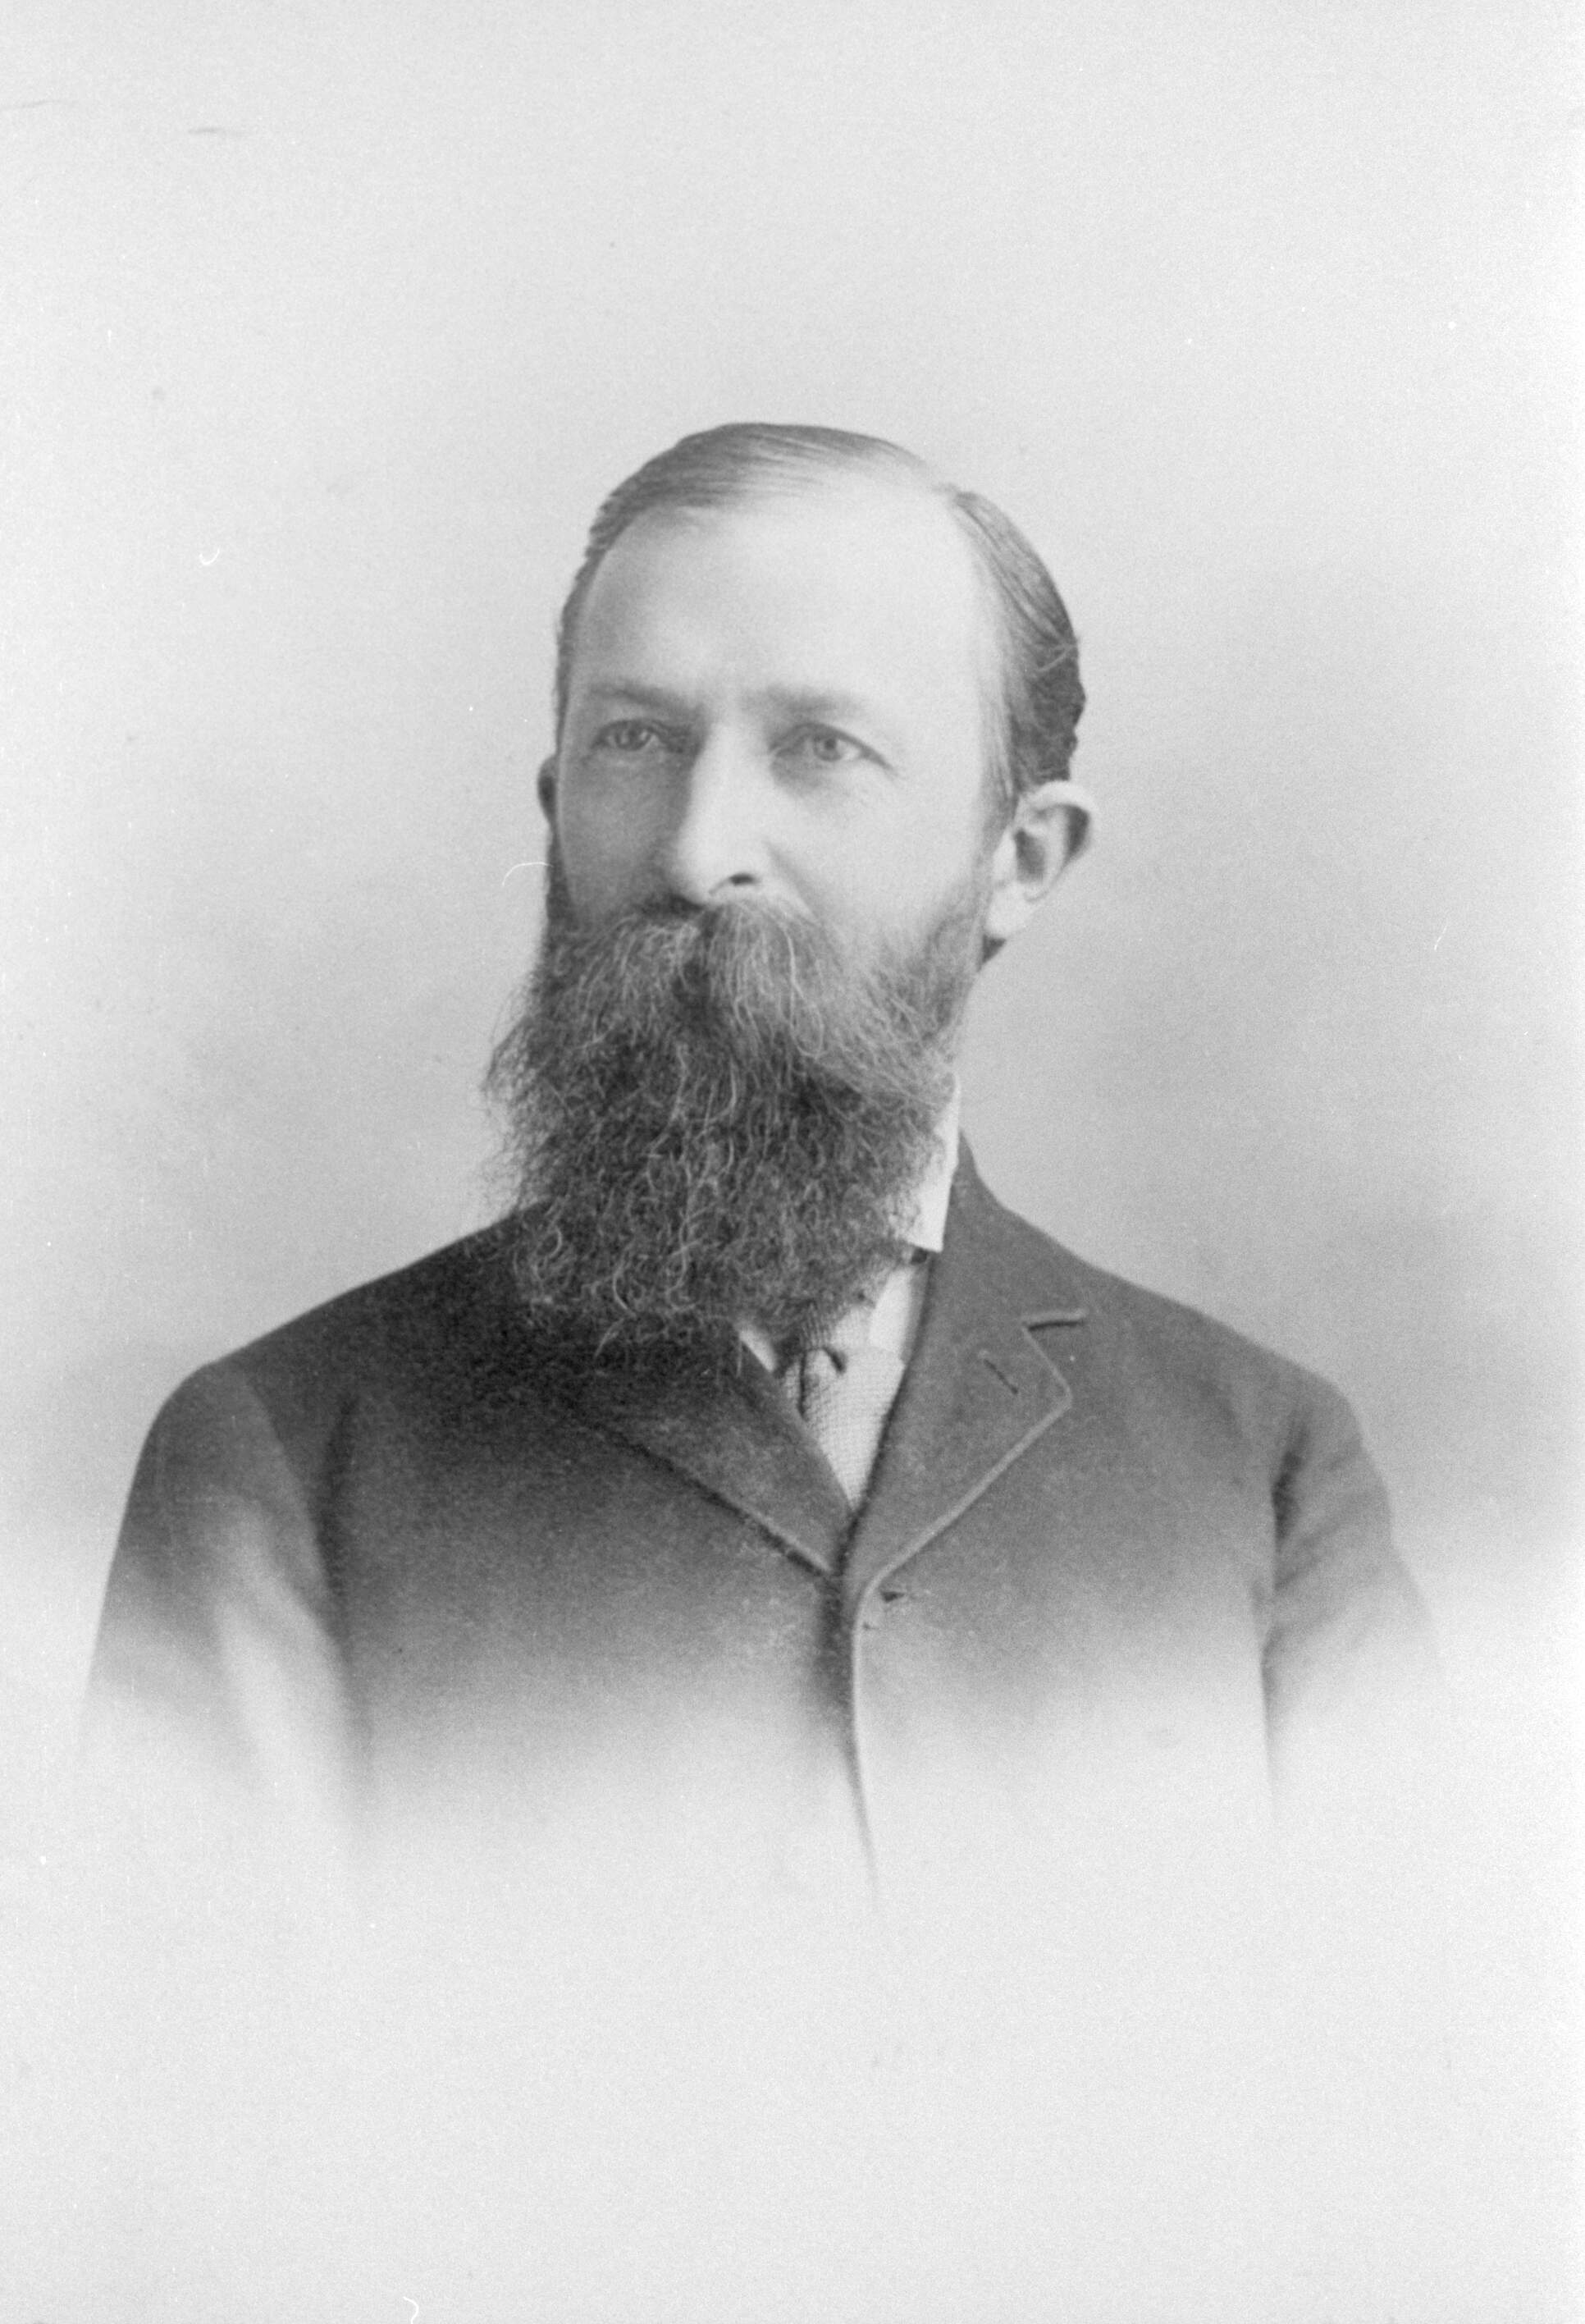
\includegraphics[width=1\linewidth]{images/john-h-kellogg.jpg}
    \caption*{John Harvey Kellogg (1852-1943)}
    \label{fig:john-h-kellogg}
\end{figure}


\begin{figure}[hp]
    \centering
    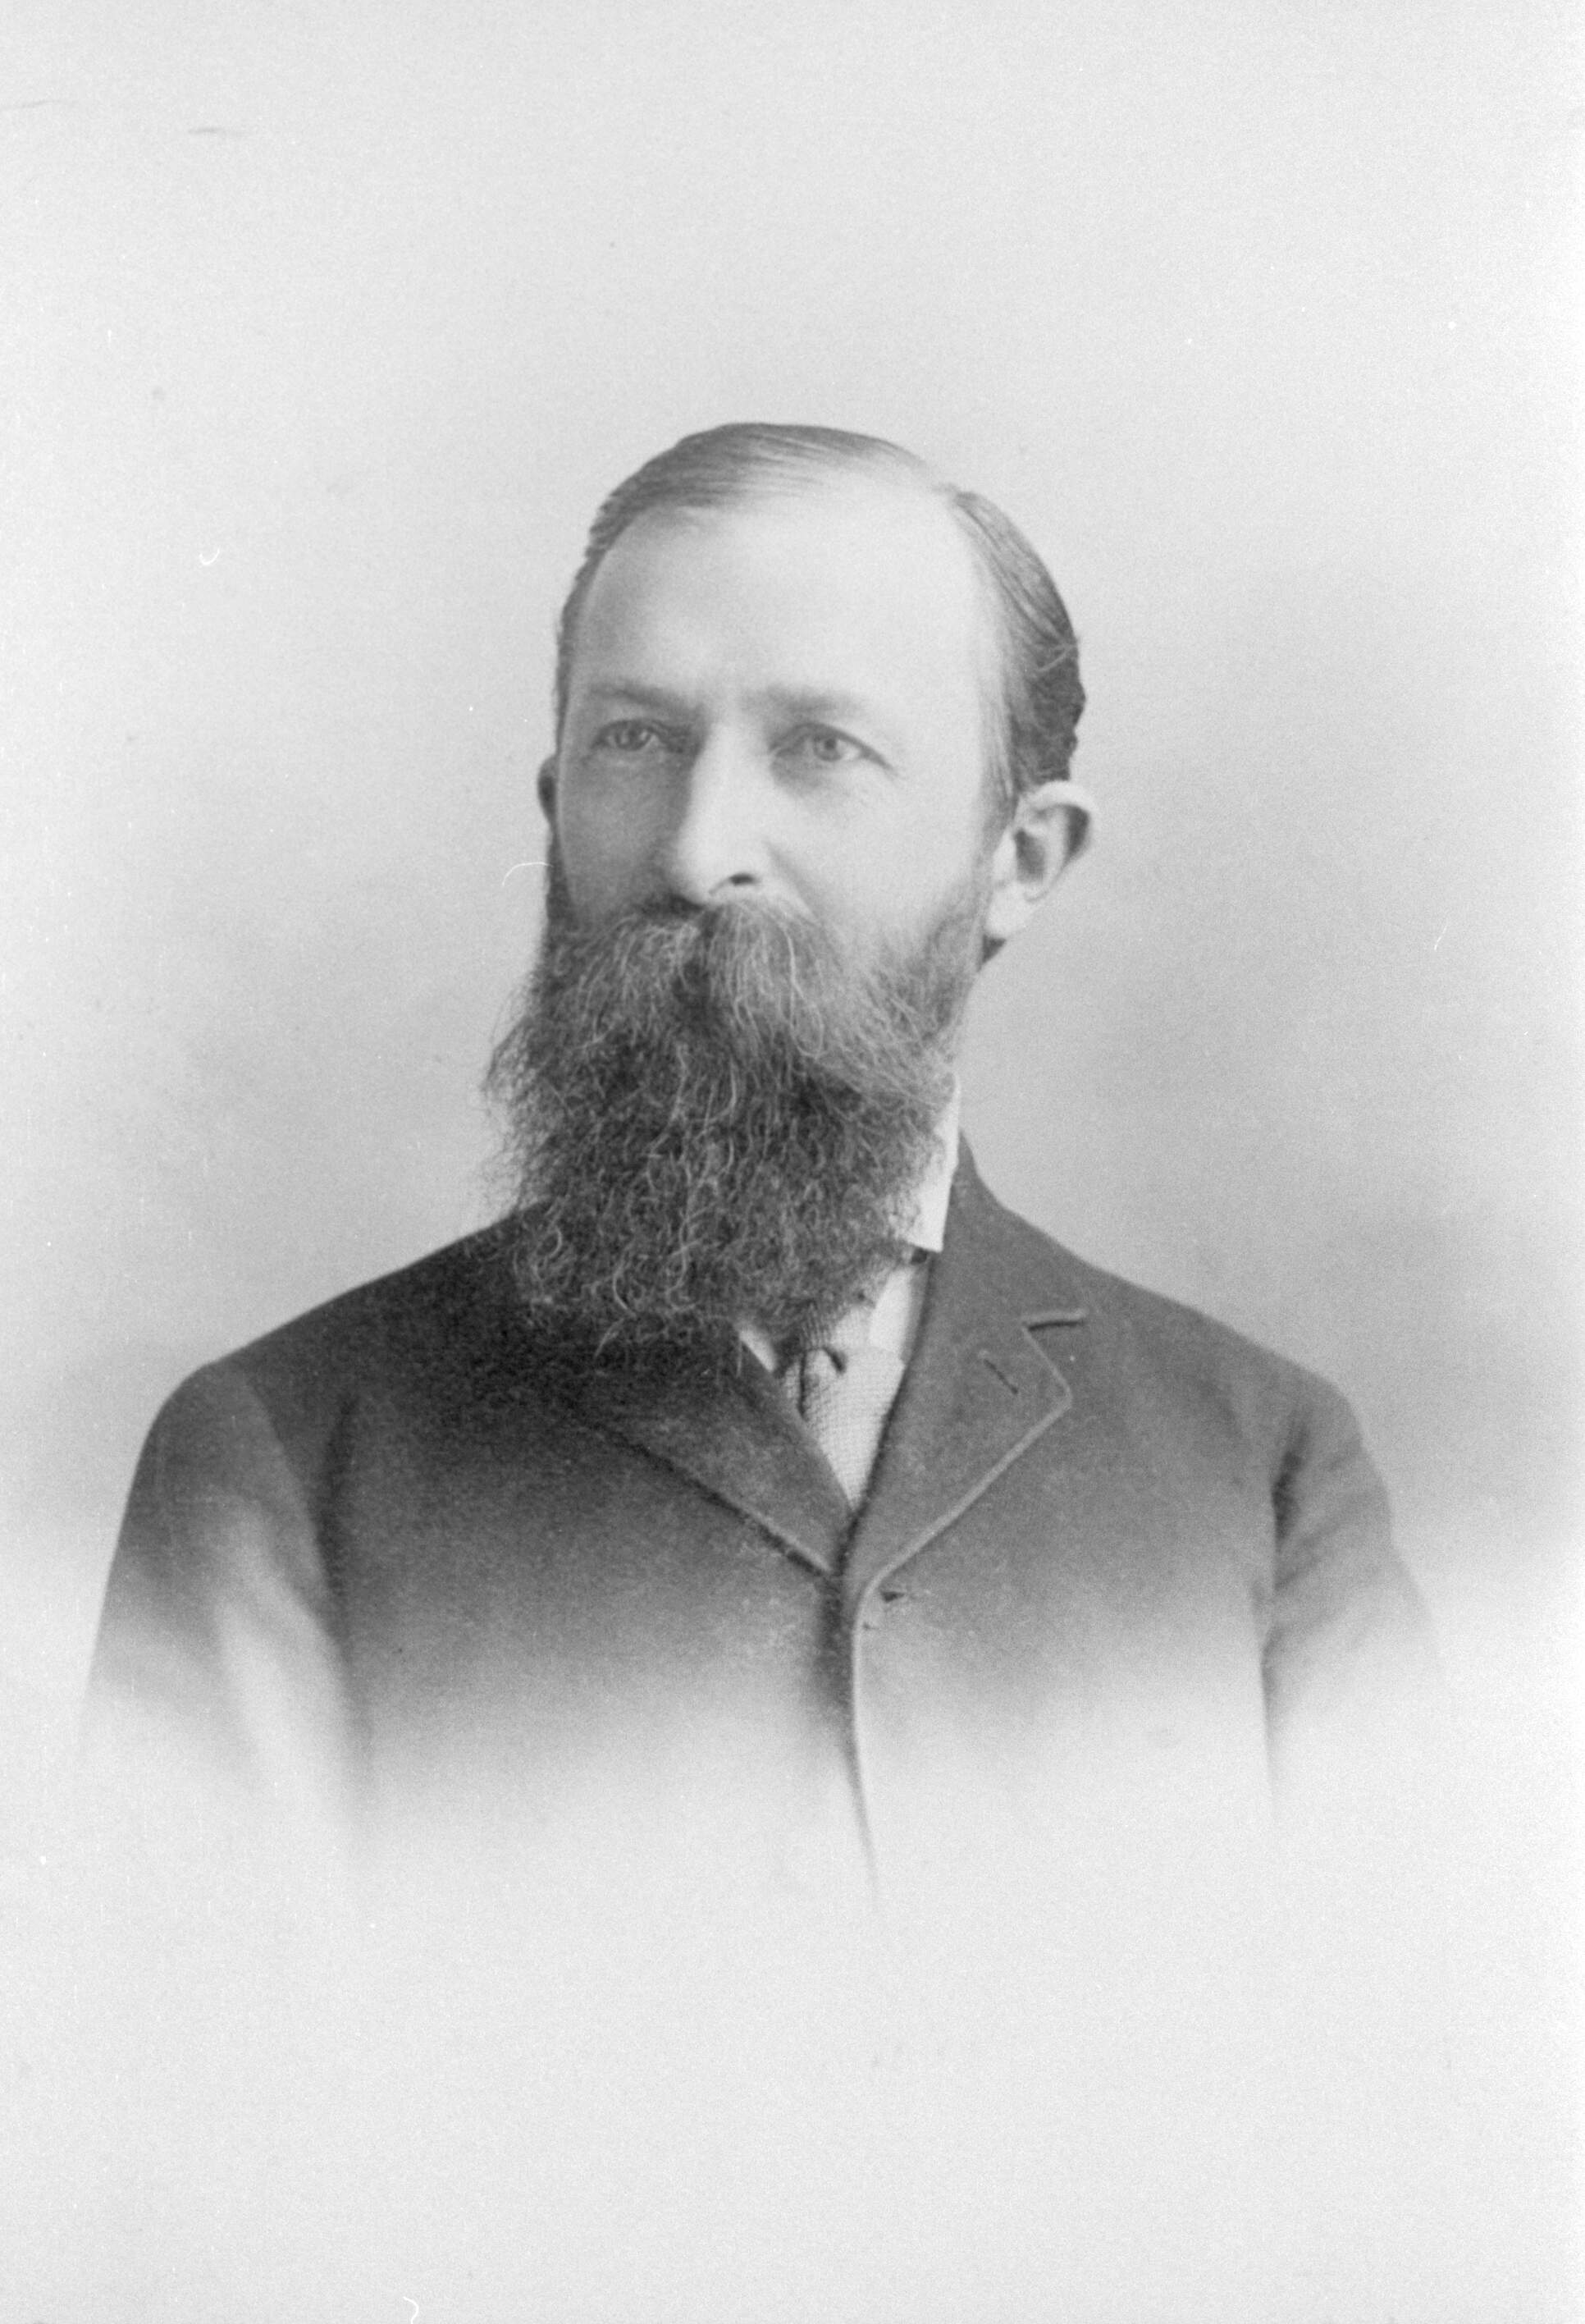
\includegraphics[width=1\linewidth]{images/john-h-kellogg.jpg}
    \caption*{John Harvey Kellogg (1852-1943)}
    \label{fig:john-h-kellogg}
\end{figure}


\egw{\textbf{The book Living Temple contains specious, \underline{deceptive sentiments regarding the personality of God and of Christ}}. The Lord opened before me the true meaning of these sentiments, showing me that unless they were steadfastly repudiated, they would deceive the very elect. \textbf{Precious truth and beautiful sentiments were woven in with false, misleading theories. Thus truth was used to substantiate the \underline{most dangerous errors}. The precious representations of God are so misconstrued as to appear to uphold falsehoods \underline{originated by the great apostate}. Sentiments that belong to the revealings of God are mingled with specious, deceptive theories of satanic agencies}.}[Lt146-1905.2; 1905][https://egwwritings.org/read?panels=p9430.8]


\egw{\textbf{El libro Living Temple contiene sentimientos especiosos, \underline{engañosos respecto a la personalidad de Dios y de Cristo}}. El Señor abrió ante mí el verdadero significado de estos sentimientos, mostrándome que, a menos que fueran firmemente repudiados, engañarían a los mismos elegidos. \textbf{La preciosa verdad y los hermosos sentimientos se entretejían con teorías falsas y engañosas. Así, la verdad fue utilizada para fundamentar los \underline{errores más peligrosos}. Las preciosas representaciones de Dios se malinterpretan de tal manera que parecen sostener falsedades \underline{originadas por el gran apóstata}. Los sentimientos que pertenecen a las revelaciones de Dios se mezclan con teorías engañosas y especiosas de los organismos satánicos}.}[Lt146-1905.2; 1905][https://egwwritings.org/read?panels=p9430.8]


\egwnogap{In the controversy over these theories \textbf{it has been asserted that I believed and taught the same things} that I have been instructed to condemn in the book Living Temple. \textbf{This I deny}. In the name of Jesus Christ of Nazareth, \textbf{I say that this is not so}.}[Lt146-1905.3; 1905][https://egwwritings.org/read?panels=p9430.9]


\egwnogap{En la controversia sobre estas teorías \textbf{se ha afirmado que yo creía y enseñaba las mismas cosas} que se me ha ordenado condenar en el libro Living Temple. \textbf{Esto lo niego}. En nombre de Jesucristo de Nazaret, \textbf{digo que no es así}.}[Lt146-1905.3; 1905][https://egwwritings.org/read?panels=p9430.9]


This mixture of truth and error makes the matter difficult. In the eyes of pro-trinitarian scholars, the problem is solely attributed to pantheism, and the evidence of Kellogg's belief in the Trinity doctrine is interpreted as belief in a false Trinity\footnote{Whidden, Woodrow W, et al. \textit{The Trinity : Understanding God's Love, His Plan of Salvation, and Christian Relationships}. Hagerstown, Md, Review And Herald Pub. Association, 2002., p. 217}. Sister White's rebuke is attributed to the defense of the “correct” Trinity, which she supposedly believed. Unfortunately, such interpretation does not acknowledge Sister White's defense of the \emcap{Fundamental Principles} regarding the \emcap{personality of God} and of Christ, thus it is a misinterpretation of her work. In the following sections, we will examine historical data on Dr. Kellogg's connection with the doctrine of Trinity from the perspective of the Adventist truth on the \emcap{personality of God}, which constituted the foundation of our faith. With this perspective, we believe that the historical data will shine in a new light and spark honest and constructive dialogue in our church.


Esta mezcla de verdad y error dificulta el asunto. A los ojos de los académicos pro-trinitarios, el problema se atribuye únicamente al panteísmo, y la evidencia de la creencia de Kellogg en la doctrina trinitaria se interpreta como una creencia en una falsa trinidad\footnote{Whidden, Woodrow W, et al. \textit{The Trinity : Understanding God's Love, His Plan of Salvation, and Christian Relationships}. Hagerstown, Md, Review And Herald Pub. Association, 2002., p. 217}. La reprimenda de la hermana White se atribuye a la defensa de la trinidad “correcta”, en la que supuestamente creía. Desgraciadamente, tal interpretación no reconoce la defensa de la hermana White de los \emcap{Principios Fundamentales} respecto a la \emcap{personalidad de Dios} y de Cristo, por lo que es una interpretación errónea de su obra. En las siguientes secciones, examinaremos los datos históricos sobre la conexión del Dr. Kellogg con la doctrina trinitaria desde la perspectiva de la verdad adventista sobre la \emcap{personalidad de Dios}, que constituyó el fundamento de nuestra fe. Con esta perspectiva, creemos que los datos históricos brillarán con una nueva luz y provocarán un diálogo honesto y constructivo en nuestra iglesia.


\section*{Correspondence of Dr. Kellogg and Brother Butler}


\section*{Correspondencia del Dr. Kellogg y el hermano Butler}


In the following section we briefly present you with the well-known correspondence between Dr. Kellogg and G. I. Butler over the book, the Living Temple. Here, we see Dr. Kellogg’s objections regarding the controversy. He wrote to Brother Butler:


En la siguiente sección les presentamos brevemente la conocida correspondencia entre el Dr. Kellogg y G. I. Butler sobre el libro, el Living Temple. Aquí vemos las objeciones del Dr. Kellogg con respecto a la controversia. Escribió al hermano Butler:


\others{As far as I can fathom, the \textbf{difficulty }which is found \textbf{in ‘The Living Temple’,} \textbf{the whole thing may be simmered down to the question}: \textbf{\underline{Is the Holy Ghost a person}?} You say no. I had supposed the Bible said this for the reason that the personal pronoun ‘he’ is used in speaking of the Holy Ghost. \textbf{Sister White uses the pronoun ‘he’ and has said in so many words that the Holy Ghost is \underline{the third person of the Godhead}}. \textbf{How the Holy Ghost can be the third person and not be a person at all is difficult for me to see}.}[Letter: J. H. Kellogg to G. I. Butler. Oct 28. 1903][https://static1.squarespace.com/static/554c4998e4b04e89ea0c4073/t/5db9fbc96defed1e45b497a4/1572469707862/1903-10-28-Kellog-to-Butler.pdf]


\others{Hasta donde puedo entender, la \textbf{dificultad} que se encuentra \textbf{en ‘The Living Temple’,} \textbf{todo el asunto puede reducirse a la pregunta}: \textbf{\underline{¿Es el Espíritu Santo una persona}?} Usted dice que no. Yo había supuesto que la Biblia decía esto por la razón de que el pronombre personal ‘él’ se utiliza al hablar del Espíritu Santo. \textbf{La hermana White usa el pronombre ‘él’ y ha dicho en muchas palabras que el Espíritu Santo es \underline{la tercera persona de la Divinidad}}. \textbf{Cómo el Espíritu Santo puede ser la tercera persona y no ser una persona en absoluto me resulta difícil de ver}.}[Letter: J. H. Kellogg to G. I. Butler. Oct 28. 1903][https://static1.squarespace.com/static/554c4998e4b04e89ea0c4073/t/5db9fbc96defed1e45b497a4/1572469707862/1903-10-28-Kellog-to-Butler.pdf]


\begin{figure}[hp]
    \centering
    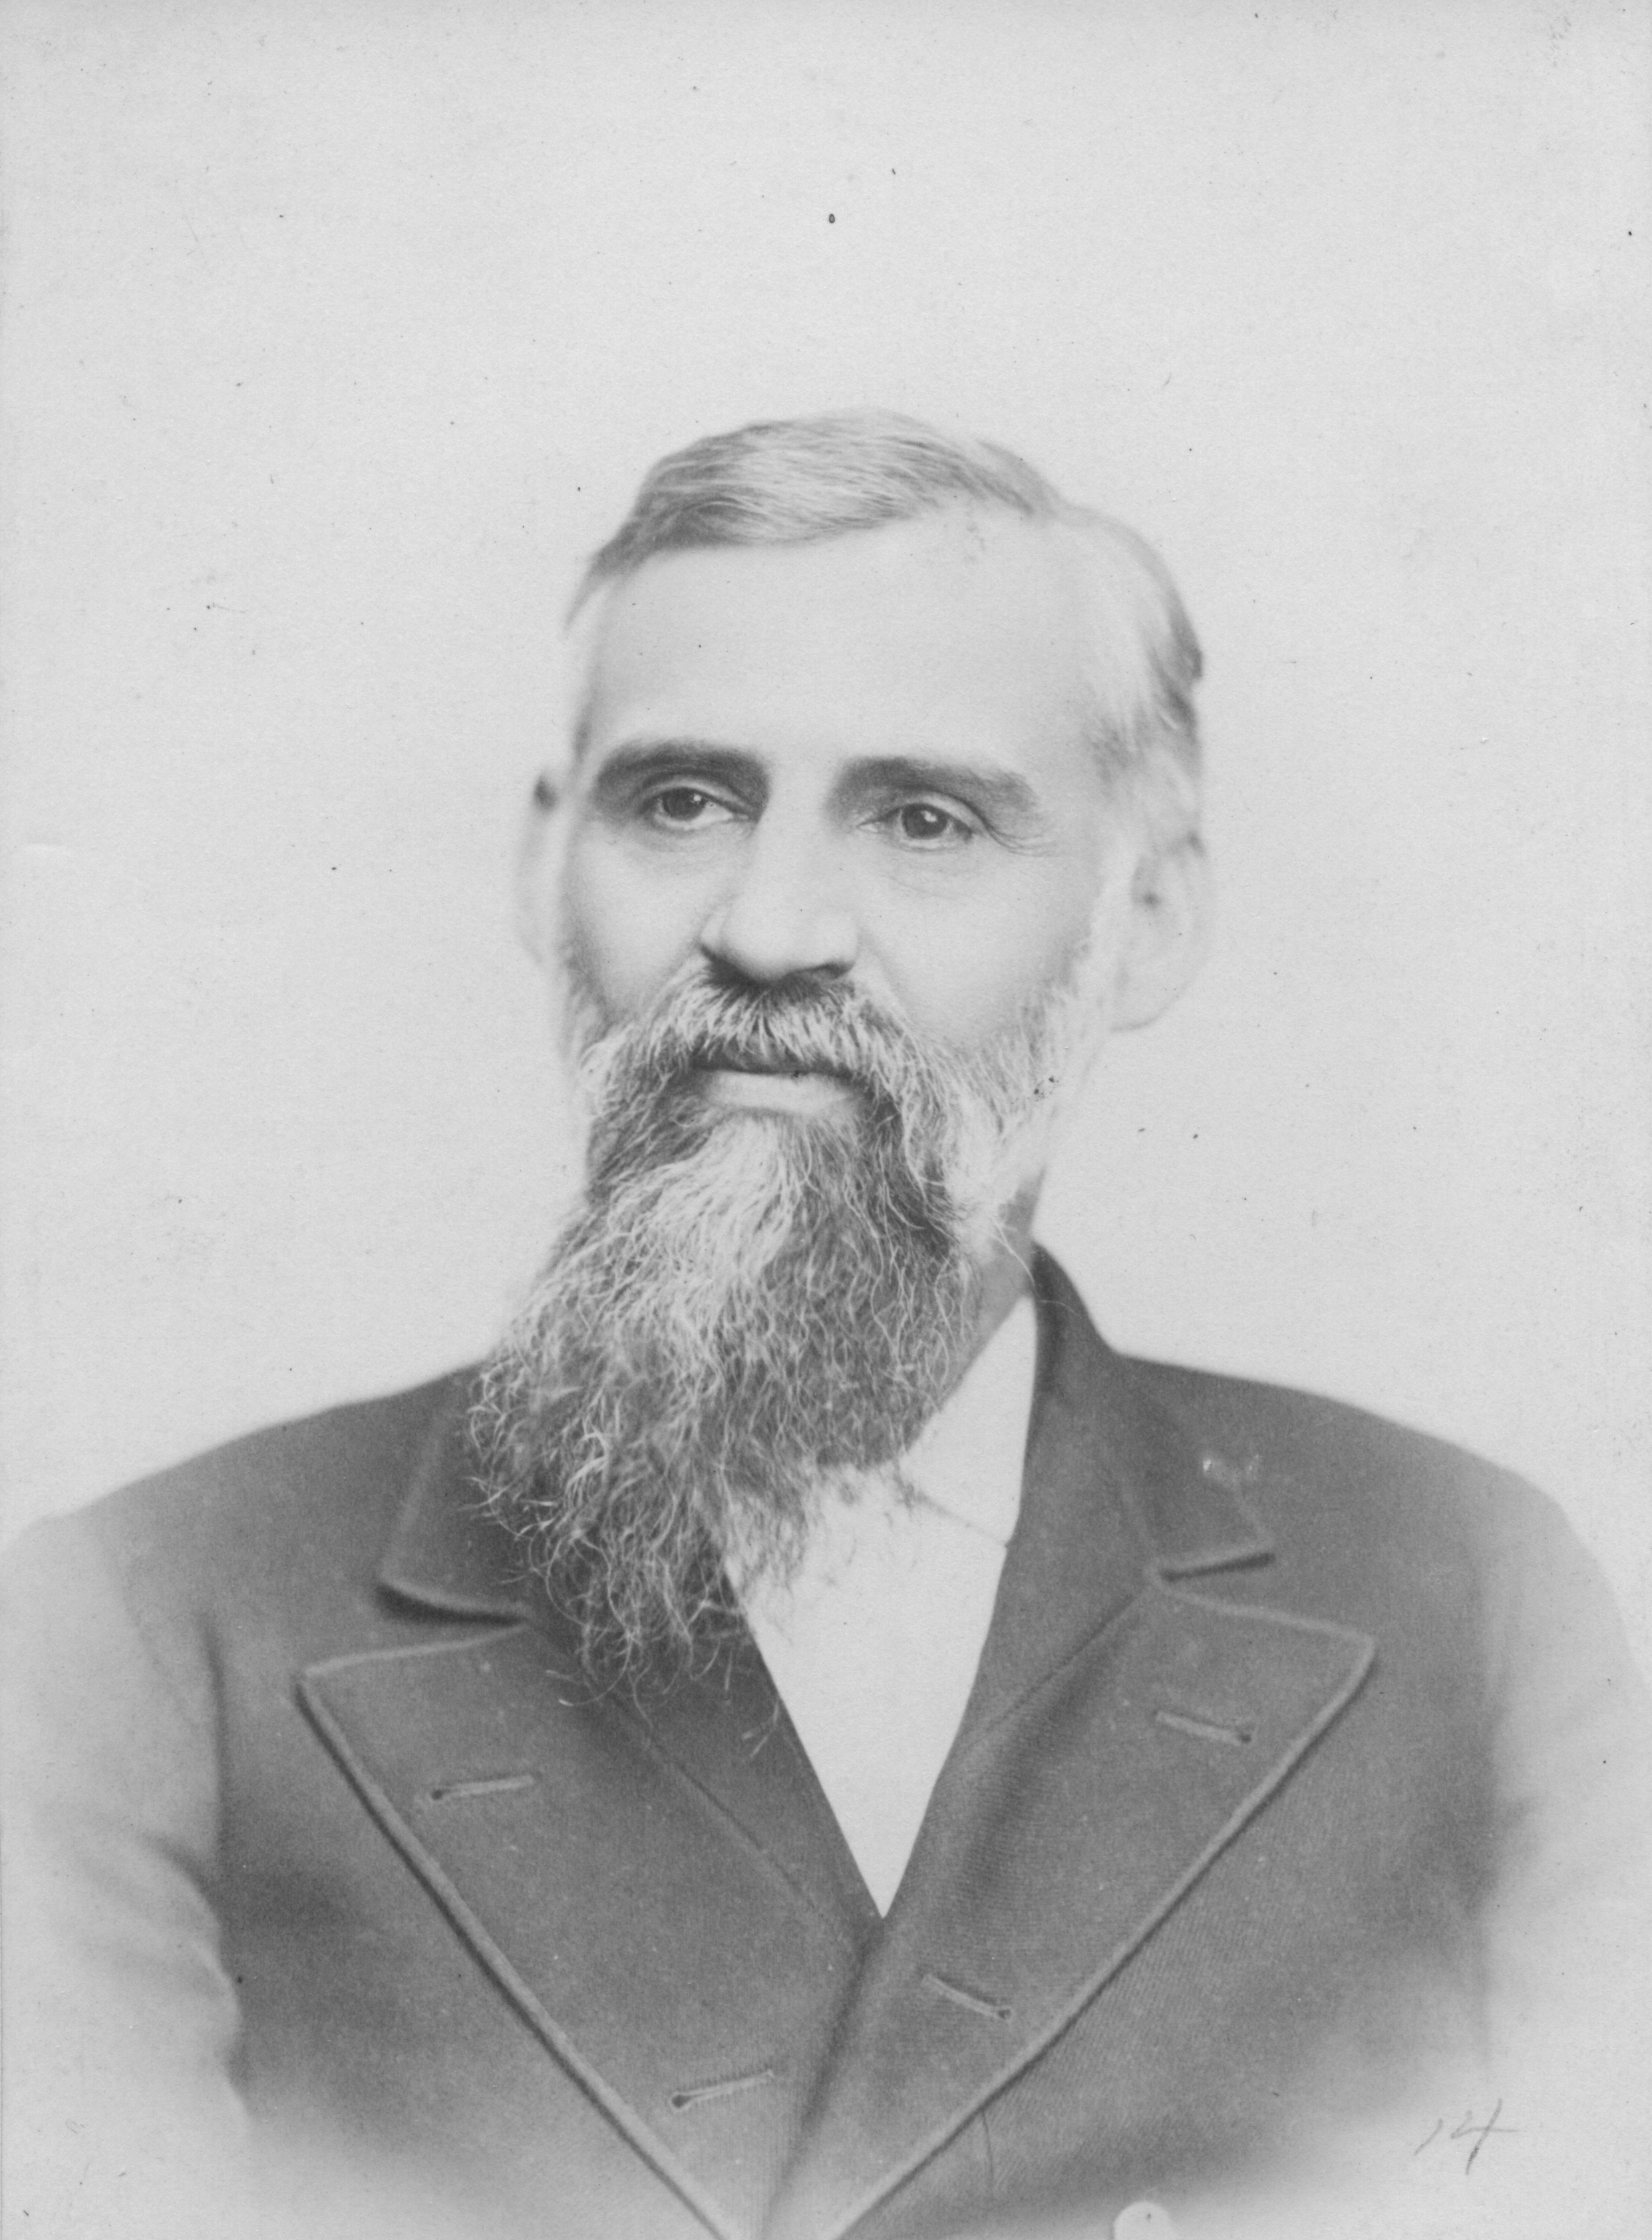
\includegraphics[width=1\linewidth]{images/george-ide-butler.jpg}
    \caption*{George Ide Butler (1834-1918)}
    \label{fig:g-i-butler}
\end{figure}


\begin{figure}[hp]
    \centering
    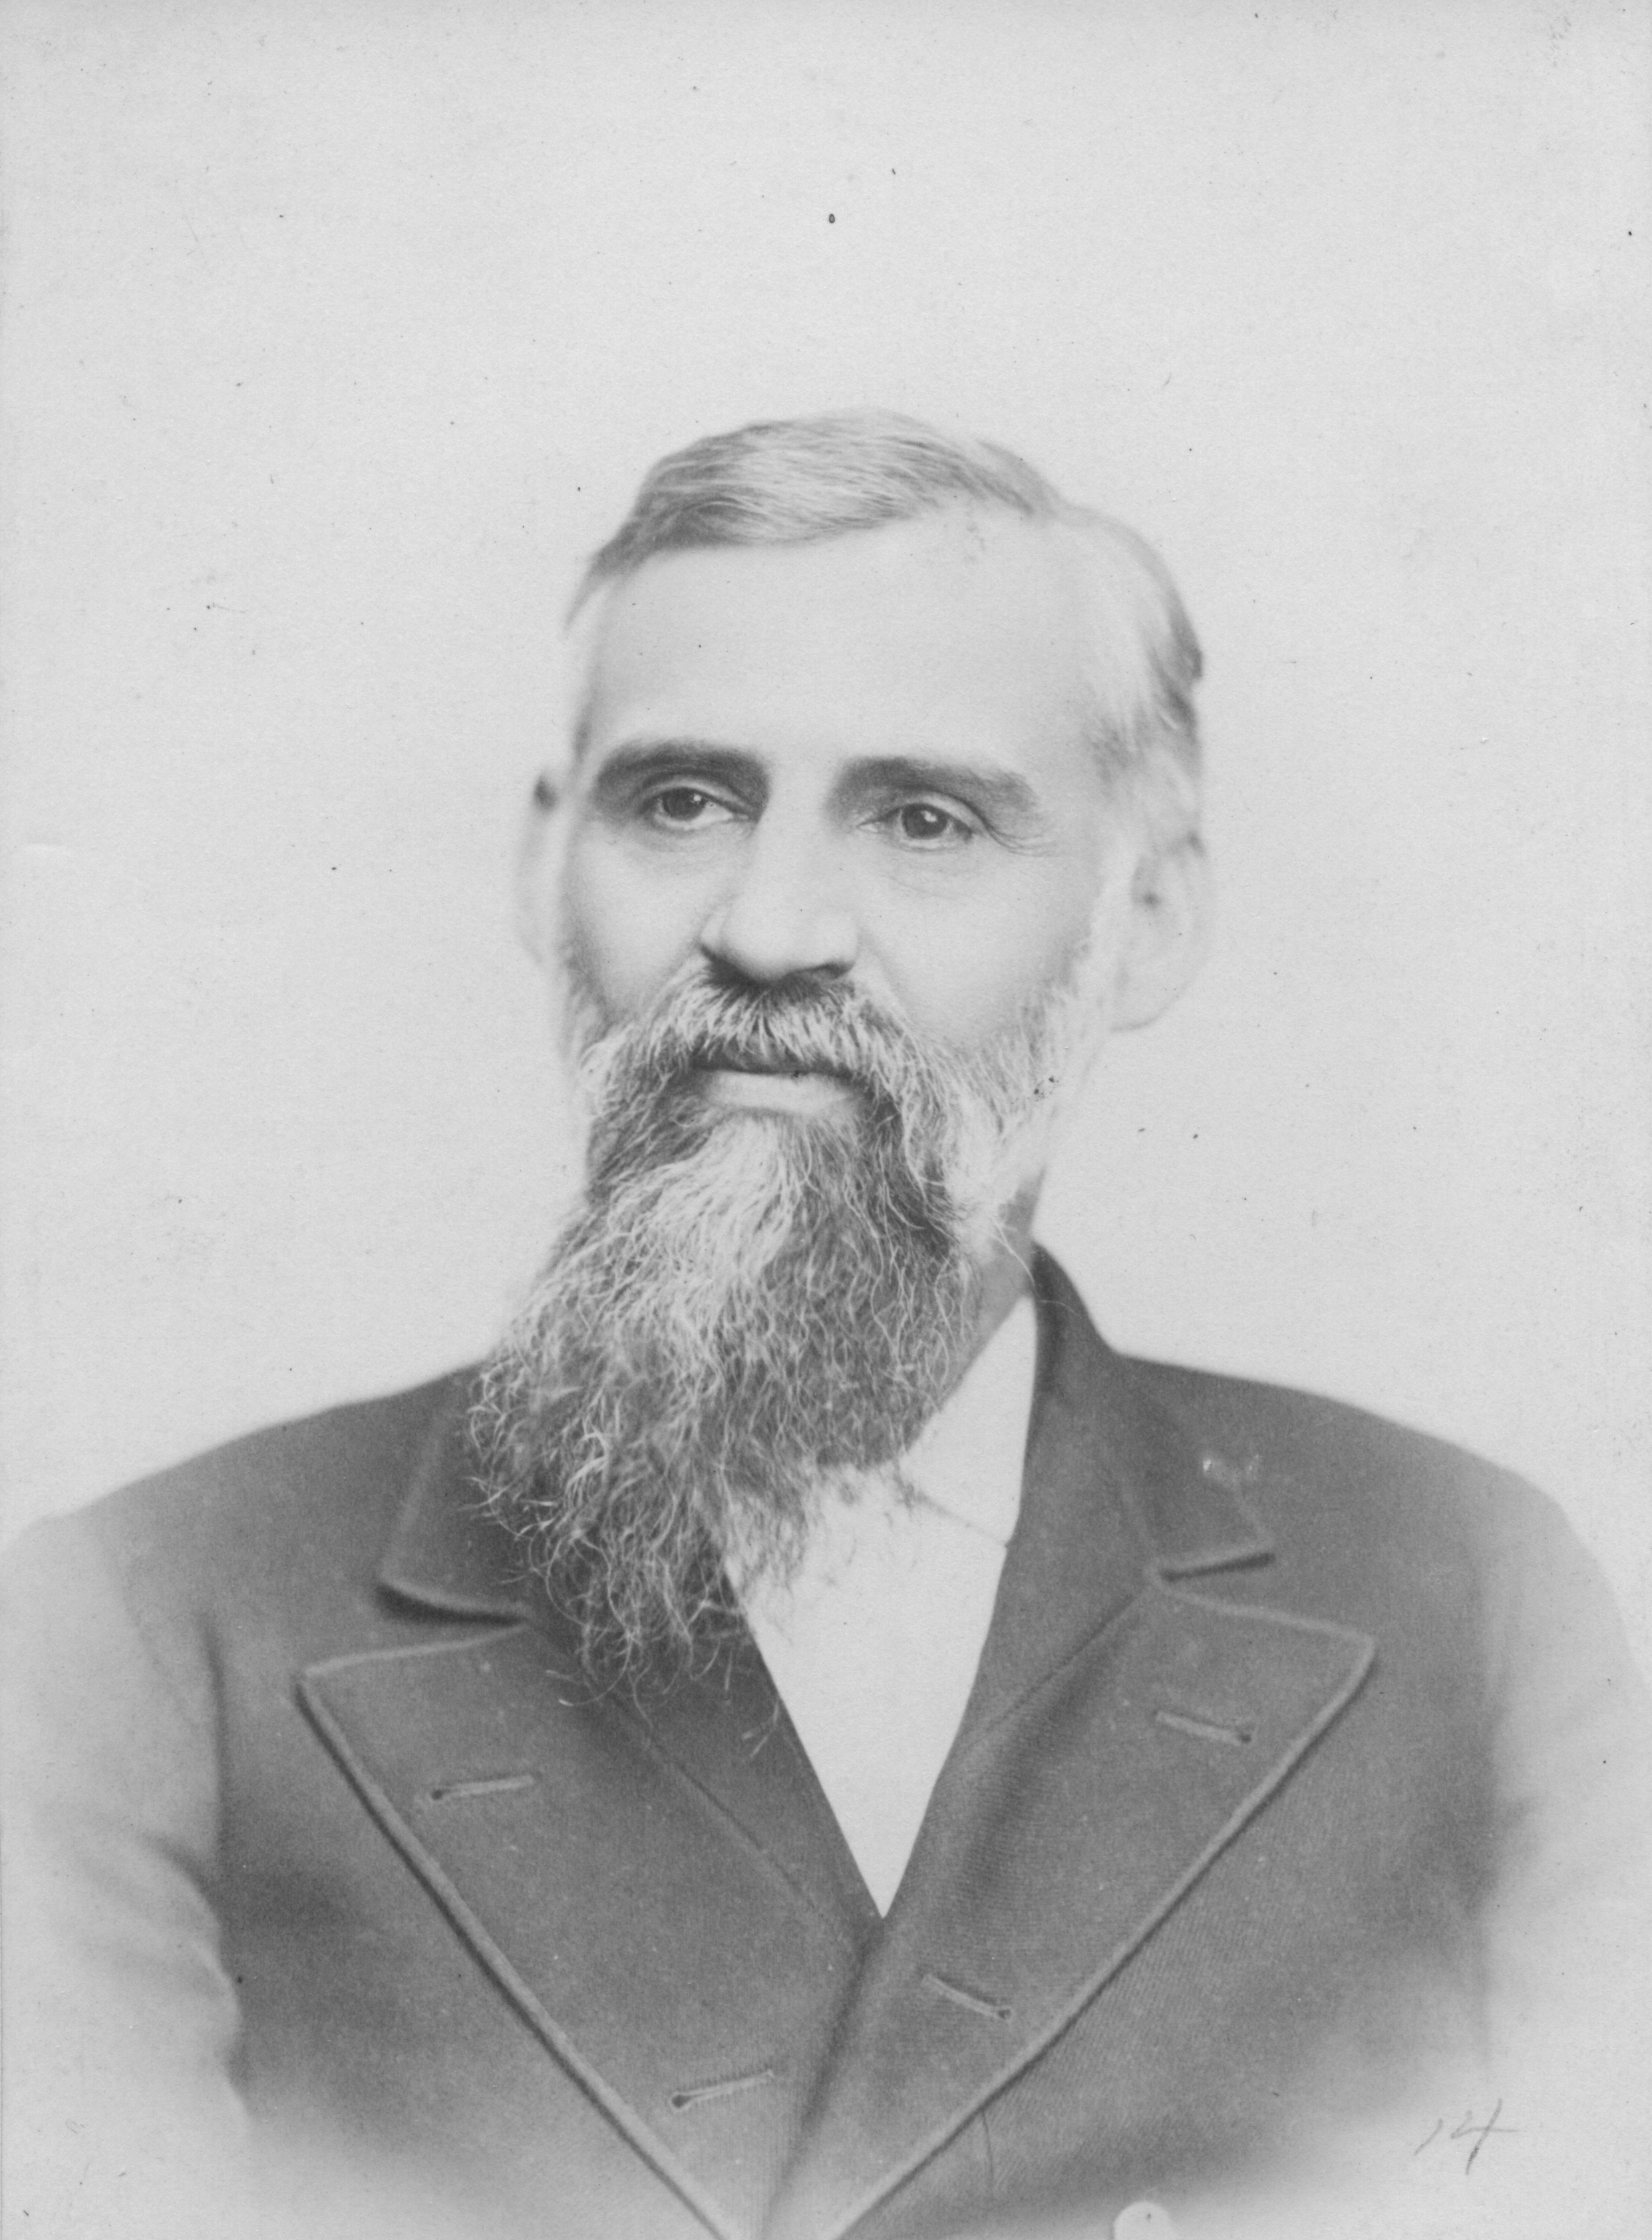
\includegraphics[width=1\linewidth]{images/george-ide-butler.jpg}
    \caption*{George Ide Butler (1834-1918)}
    \label{fig:g-i-butler}
\end{figure}


According to Dr. Kellogg’s perspective, the whole problem with the book ‘The Living Temple’ comes down to the question “\textit{Is the Holy Ghost a person?}”. Obviously, he does not advocate an impersonal God, as he is often accused of\footnote{Whidden, Woodrow W, et al. \textit{The Trinity : Understanding God's Love, His Plan of Salvation, and Christian Relationships}. Hagerstown, Md, Review And Herald Pub. Association, 2002., p. 217}. Moreover, he even believes that the Holy Ghost is a \textit{third person of the Godhead}. Also, he claims that Brother Butler does not believe that the Holy Ghost is a person. The problem obviously lies in the definition of the word \textit{‘person’}. On this point, Kellogg continues:


Según la perspectiva del Dr. Kellogg, todo el problema del libro ‘El Templo Viviente’ se reduce a la pregunta “\textit{¿Es el Espíritu Santo una persona?}”. Obviamente, él no defiende un Dios impersonal, como se le acusa a menudo\footnote{Whidden, Woodrow W, et al. \textit{The Trinity : Understanding God's Love, His Plan of Salvation, and Christian Relationships}. Hagerstown, Md, Review And Herald Pub. Association, 2002., p. 217}. Es más, incluso cree que el Espíritu Santo es una \textit{tercera persona de la Divinidad}. Además, afirma que el hermano Butler no cree que el Espíritu Santo sea una persona. El problema radica obviamente en la definición de la palabra \textit{‘persona’}. Sobre este punto, Kellogg continúa:


\others{I believe this Spirit of God to be a personality you don’t. But this is purely a question of definition. \textbf{I believe the Spirit of God is a personality}; you say, No, it is not a personality. Now the only reason why we differ is because we \textbf{differ in our ideas as to \underline{what a personality is}}. \textbf{Your idea of personality is perhaps that of \underline{semblance to a person} or a human being}.}[Letter: J. H. Kellogg to G. I. Butler. Oct 28. 1903][https://static1.squarespace.com/static/554c4998e4b04e89ea0c4073/t/5db9fbc96defed1e45b497a4/1572469707862/1903-10-28-Kellog-to-Butler.pdf]


\others{Yo creo que este Espíritu de Dios es una personalidad que tú no crees. Pero esto es puramente una cuestión de definición. \textbf{Yo creo que el Espíritu de Dios es una personalidad}; tú dices que no, que no es una personalidad. Ahora, la única razón por la que diferimos es porque \textbf{diferimos en nuestras ideas sobre \underline{lo que es una personalidad}}. \textbf{Tu idea de personalidad es quizás la de \underline{apariencia de una persona} o un ser humano}.}[Letter: J. H. Kellogg to G. I. Butler. Oct 28. 1903][https://static1.squarespace.com/static/554c4998e4b04e89ea0c4073/t/5db9fbc96defed1e45b497a4/1572469707862/1903-10-28-Kellog-to-Butler.pdf]


Brother Butler replied:


El hermano Butler respondió:


\others{\textbf{So far as Sister White and you being in perfect agreement, I shall have to leave that entirely between you and Sister White. \underline{Sister White says there is not perfect agreement; you claim there is}. \underline{I know some of her remarks seem to give you strong ground for claiming that she does}. I am candid enough to say that, but I must give her the credit until she disowns it of saying there is a difference too, and I do not believe you can fully tell just what she means. \underline{God dwells in us by His Holy Spirit}, as a Comforter, as a Reprover, especially the former. When we come to Him we partake of Him in that sense, because the Spirit comes forth from Him; \underline{it comes forth from the Father and the Son}. It is not a person walking around on foot, or flying \underline{as a literal being}, \underline{in any such sense as Christ and the Father are} – at least, if it is, it is utterly beyond my comprehension of the meaning of language or words}.}[Letter: G. I. Butler to J. H. Kellogg. April 5. 1904]


\others{\textbf{En cuanto a que la hermana White y usted estén en perfecto acuerdo, tendré que dejar eso totalmente entre usted y la hermana White. \underline{La hermana White dice que no hay un acuerdo perfecto; usted afirma que sí lo hay}. \underline{Sé que algunos de sus comentarios parecen darle a usted una base sólida para afirmar que sí lo hay}. Soy lo suficientemente sincero como para decir eso, pero debo darle el crédito, hasta que ella lo desmienta, de decir que también hay una diferencia, y no creo que usted pueda decir completamente lo que ella quiere decir. \underline{Dios mora en nosotros por medio de su Espíritu Santo}, como Consolador, como Reprobador, especialmente el primero. Cuando venimos a Él, participamos de Él en ese sentido, porque el Espíritu sale de Él; \underline{sale del Padre y del Hijo}. No es una persona que camina a pie, o que vuela \underline{como un ser literal}, \underline{en ningún sentido como lo son Cristo y el Padre} – al menos, si lo es, está totalmente más allá de mi comprensión del significado del lenguaje o palabras}.}[Letter: G. I. Butler to J. H. Kellogg. April 5. 1904]


The given correspondence is crucial for understanding the Kellogg controversy. Kellogg himself stated, \others{the whole thing may be simmered down to the question: \textbf{Is the Holy Ghost a person?}} Similarly Dr. Kellogg wrote to William White: \others{I have been studying very carefully to see what is \textbf{the real root of the difficulty with the Living Temple}, and as far as I can see \textbf{\underline{the whole question} resolves itself into this: \underline{Is the Holy Ghost, a person}?}}[Letter J. H. Kellogg to William White, October 28, 1903][https://drive.google.com/file/d/1\_S4S-Hc0K7Ka8gda9oRhPuAb9XzBTwmb/view] How does Kellogg's conclusion compare to the review and instruction of heavenly origin, which clearly told us that the reasoning in the Living Temple is \egwinline{naught but speculation in regard to \textbf{the personality of God and where His presence is}}[SpTB02 51.3; 1904][https://egwwritings.org/read?panels=p417.262]? In the writings of Ellen White and the pioneers, the term ‘\textit{personality of God}’ refers specifically to the personality of the Father. So, why does Kellogg claim that the real issue is the personality of the Holy Spirit, when God indicated that the issue concerns the personality of the Father?


La correspondencia dada es crucial para entender la controversia de Kellogg. El mismo Kellogg declaró, \others{todo el asunto puede reducirse a la pregunta: \textbf{¿Es el Espíritu Santo una persona?}} De manera similar, el Dr. Kellogg escribió a William White: \others{He estado estudiando muy cuidadosamente para ver cuál es \textbf{la verdadera raíz de la dificultad con el Templo Viviente}, y hasta donde puedo ver \textbf{\underline{toda la cuestión} se reduce a esto: \underline{¿Es el Espíritu Santo una persona}?}}[Letter J. H. Kellogg to William White, October 28, 1903][https://drive.google.com/file/d/1\_S4S-Hc0K7Ka8gda9oRhPuAb9XzBTwmb/view] ¿Cómo se compara la conclusión de Kellogg con la revisión e instrucción de origen celestial, que claramente nos dijo que el razonamiento en el Templo Viviente es \egwinline{nada más que especulación con respecto a \textbf{la personalidad de Dios y dónde está Su presencia}}[SpTB02 51.3; 1904][https://egwwritings.org/read?panels=p417.262]? En los escritos de Elena de White y los pioneros, el término ‘\textit{personalidad de Dios}’ se refiere específicamente a la personalidad del Padre. Entonces, ¿por qué Kellogg afirma que el verdadero problema es la personalidad del Espíritu Santo, cuando Dios indicó que el problema concierne a la personalidad del Padre?


Many assume that Dr. Kellogg is being manipulative, evading the core issue. However, under a particular premise, his arguments concerning the personality of the Holy Spirit logically support his controversial views on the \emcap{personality of God}. This premise becomes evident within the data itself when we closely follow his reasoning.


Muchos asumen que el Dr. Kellogg está siendo manipulador, evadiendo el problema central. Sin embargo, bajo una premisa particular, sus argumentos concernientes a la personalidad del Espíritu Santo apoyan lógicamente sus controvertidas opiniones sobre la \emcap{personalidad de Dios}. Esta premisa se hace evidente dentro de los datos mismos cuando seguimos de cerca su razonamiento.


As we have seen earlier, the doctrine on the \emcap{personality of God} teaches that God, the Father, possesses a form—a tangible, material body. Dr. Kellogg concurred that this assertion holds true within the bounds of our finite conception of God\footnote{\href{https://archive.org/details/J.H.Kellogg.TheLivingTemple1903/page/n33/}{Dr. John H. Kellogg, The Living Temple, p.31.}}. However, he argued that, in reality, God transcends our conceptions regarding His form, as He is beyond the constraints of space\footnote{\href{https://archive.org/details/J.H.Kellogg.TheLivingTemple1903/page/n33/}{Dr. John H. Kellogg, The Living Temple, p.33.}}. In this sense, Kellogg effectively does away with the reality of God’s physical, material body. The premise that would validate Dr. Kellogg’s viewpoint is the \textit{exclusive equivalence} in understanding the \emcap{personality of God} and that of the Holy Spirit. Is the Holy Spirit constrained by space? No, He is not. Does the Holy Spirit have a physical body? No! According to Jesus, \bible{for a spirit hath not flesh and bones}[Luke 24:39]. Is the Holy Ghost a person? The answer hinges on our interpretation of what it means to be a person. What is that quality or state of the Holy Spirit being a person?\footnote{Direct application of the definition on the word ‘\textit{personality}’ from the \href{https://www.merriam-webster.com/dictionary/personality}{Merriam Webster Dictionary}} When comparing Dr. Kellogg's belief in the personality of the Holy Spirit with Brother Butler's views, it becomes evident that the quality of the Holy Spirit being a person does not align with \others{that of \textbf{semblance to a person} or a human being}. Butler explicitly stated his criteria for this determination\footnote{In his letter to Dr. Kellogg, Brother Butler further asserted that there is no distinction between the person and the bodily presence. See \href{https://c7da.us/egwdl/Butler\%20to\%20Kellogg\%20Aug121904.pdf}{Letter from Butler to Kellogg, August 12, 1904, p.6}}: \others{\textbf{It is not a person walking around on foot, or flying \underline{as a literal being}, \underline{in any such sense as Christ and the Father are} – at least, if it is, it is utterly beyond my comprehension of the meaning of language or words}}.


Como hemos visto anteriormente, la doctrina sobre la \emcap{personalidad de Dios} enseña que Dios, el Padre, posee una forma—un cuerpo tangible y material. El Dr. Kellogg coincidió en que esta afirmación es válida dentro de los límites de nuestra concepción finita de Dios\footnote{\href{https://archive.org/details/J.H.Kellogg.TheLivingTemple1903/page/n33/}{Dr. John H. Kellogg, The Living Temple, p.31.}}. Sin embargo, argumentó que, en realidad, Dios trasciende nuestras concepciones respecto a Su forma, ya que está más allá de las limitaciones del espacio\footnote{\href{https://archive.org/details/J.H.Kellogg.TheLivingTemple1903/page/n33/}{Dr. John H. Kellogg, The Living Temple, p.33.}}. En este sentido, Kellogg efectivamente elimina la realidad del cuerpo físico y material de Dios. La premisa que validaría el punto de vista del Dr. Kellogg es la \textit{equivalencia exclusiva} en la comprensión de la \emcap{personalidad de Dios} y la del Espíritu Santo. ¿Está el Espíritu Santo limitado por el espacio? No, no lo está. ¿Tiene el Espíritu Santo un cuerpo físico? ¡No! Según Jesús, \bible{porque un espíritu no tiene carne ni huesos}[Lucas 24:39]. ¿Es el Espíritu Santo una persona? La respuesta depende de nuestra interpretación de lo que significa ser una persona. ¿Cuál es esa cualidad o estado del Espíritu Santo siendo una persona?\footnote{Aplicación directa de la definición de la palabra ‘\textit{personalidad}’ del \href{https://www.merriam-webster.com/dictionary/personality}{Diccionario Merriam Webster}} Al comparar la creencia del Dr. Kellogg en la personalidad del Espíritu Santo con las opiniones del hermano Butler, se hace evidente que la cualidad del Espíritu Santo siendo una persona no se alinea con \others{la de \textbf{apariencia de una persona} o un ser humano}. Butler declaró explícitamente sus criterios para esta determinación\footnote{En su carta al Dr. Kellogg, el hermano Butler afirmó además que no hay distinción entre la persona y la presencia corporal. Ver \href{https://c7da.us/egwdl/Butler\%20to\%20Kellogg\%20Aug121904.pdf}{Carta de Butler a Kellogg, 12 de agosto de 1904, p.6}}: \others{\textbf{No es una persona que camina a pie, o que vuela \underline{como un ser literal}, \underline{en ningún sentido como lo son Cristo y el Padre} – al menos, si lo es, está totalmente más allá de mi comprensión del significado del lenguaje o palabras}}.


Have you noticed that Brother Butler addressed Kellogg’s unspoken premise? Butler drew a distinction between the Father and Christ, in relation to the Holy Spirit. Brother Butler is correct. There exists a contrast between the personality of the Holy Spirit and that of God and Christ. Christ and the Father possess a physical form of a person, whereas the Holy Spirit does not. To do away with the physical form of a person of the Father is to \textit{exclusively equate} the understanding of the personality of the Father with that of the Holy Spirit. Kellogg’s approach is compelling, because it was backed by valid arguments regarding the personality of the Holy Spirit.


¿Has notado que el hermano Butler abordó la premisa no expresada de Kellogg? Butler estableció una distinción entre el Padre y Cristo, en relación con el Espíritu Santo. El hermano Butler tiene razón. Existe un contraste entre la personalidad del Espíritu Santo y la de Dios y Cristo. Cristo y el Padre poseen una forma física de persona, mientras que el Espíritu Santo no. Eliminar la forma física de la persona del Padre es \textit{equiparar exclusivamente} la comprensión de la personalidad del Padre con la del Espíritu Santo. El enfoque de Kellogg es convincente, porque estaba respaldado por argumentos válidos sobre la personalidad del Espíritu Santo.


Let us briefly examine the personality of the Holy Spirit. What is the quality or state of the Holy Spirit being a person?


Examinemos brevemente la personalidad del Espíritu Santo. ¿Cuál es la cualidad o estado del Espíritu Santo siendo una persona?


\egw{\textbf{The Holy Spirit has a personality}, \textbf{\underline{else} }He could not \textbf{bear witness} to our spirits and with our spirits that we are the children of God. \textbf{He must also be a \underline{divine person}}, \textbf{\underline{else}} He could not \textbf{search out the secrets} which lie hidden \textbf{in the mind of God}.}[21LtMs, Ms 20, 1906, par. 32; 1906][https://egwwritings.org/read?panels=p14071.10296041&index=0]


\egw{\textbf{El Espíritu Santo tiene una personalidad}, \textbf{\underline{de lo contrario} }no podría \textbf{dar testimonio} a nuestros espíritus y con nuestros espíritus de que somos hijos de Dios. \textbf{También debe ser una \underline{persona divina}}, \textbf{\underline{de lo contrario}} no podría \textbf{escudriñar los secretos} que están ocultos \textbf{en la mente de Dios}.}[21LtMs, Ms 20, 1906, par. 32; 1906][https://egwwritings.org/read?panels=p14071.10296041&index=0]


\egw{\textbf{The Holy Spirit is a person}; \textbf{\underline{for}} He \textbf{beareth witness} with our spirits that we are the children of God.}[21LtMs, Ms 20, 1906, par. 31; 1906][https://egwwritings.org/read?panels=p14071.10296040&index=0]


\egw{\textbf{El Espíritu Santo es una persona}; \textbf{\underline{porque}} Él \textbf{da testimonio} con nuestros espíritus de que somos hijos de Dios.}[21LtMs, Ms 20, 1906, par. 31; 1906][https://egwwritings.org/read?panels=p14071.10296040&index=0]


The qualities or states that define the Holy Spirit as a person are explicitly mentioned in the provided quotations. These include the ability to bear witness and search out the mind. Further support can be found in Scripture, which attributes actions to the Holy Spirit such as speaking (\textit{Acts 13:2}), teaching (\textit{John 14:26; 1 Corinthians 2:13}), making decisions (\textit{Acts 15:28}), and experiencing emotions (\textit{Ephesians 4:30}), among others. These \textit{qualities }collectively affirm the personality of the Holy Spirit. Can these same qualities be also applied to the Father and the Son? Most certainly. However, unlike the Father and the Son, the Holy Spirit is distinguished by the absence of a material, tangible form. When Ellen White questioned Christ about the \emcap{personality of God}, her inquiry specifically targeted the personal form as the defining quality of the Father's personality.


Las cualidades o estados que definen al Espíritu Santo como una persona se mencionan explícitamente en las citas proporcionadas. Estas incluyen la capacidad de dar testimonio y escudriñar la mente. Se puede encontrar más apoyo en las Escrituras, que atribuyen acciones al Espíritu Santo como hablar (\textit{Hechos 13:2}), enseñar (\textit{Juan 14:26; 1 Corintios 2:13}), tomar decisiones (\textit{Hechos 15:28}), y experimentar emociones (\textit{Efesios 4:30}), entre otras. Estas \textit{cualidades} afirman colectivamente la personalidad del Espíritu Santo. ¿Pueden estas mismas cualidades aplicarse también al Padre y al Hijo? Ciertamente. Sin embargo, a diferencia del Padre y del Hijo, el Espíritu Santo se distingue por la ausencia de una forma material y tangible. Cuando Elena de White preguntó a Cristo sobre la \emcap{personalidad de Dios}, su indagación se dirigía específicamente a la forma personal como la cualidad definitoria de la personalidad del Padre.


\egw{I have often \textbf{seen }the lovely Jesus, that \textbf{He is a person}. \textbf{I asked Him if His Father \underline{was a person} and \underline{had a form} like Himself}. Said Jesus, ‘\textbf{I am in the express image of My Father's person}.’}[EW 77.1; 1882][https://egwwritings.org/read?panels=p28.490&index=0]


\egw{A menudo he \textbf{visto} al amable Jesús, que \textbf{Él es una persona}. \textbf{Le pregunté si Su Padre \underline{era una persona} y \underline{tenía una forma} como Él mismo}. Dijo Jesús: ‘\textbf{Yo soy la imagen misma de la persona de Mi Padre}’.}[EW 77.1; 1882][https://egwwritings.org/read?panels=p28.490&index=0]


This brings us to a profound distinction in how the personality of the Holy Spirit is understood, as opposed to that of the Father and the Son. Ellen White describes the Holy Spirit as a spiritual manifestation of Christ, drawing a clear line between the outward, visible manifestation of Christ and His spiritual manifestation. This contrast underscores the unique nature of the Holy Spirit's presence and action in the world, distinct from the physical presence of Christ and the Father. Pay attention to the contrast between the outward, visible manifestation of Christ, and His spiritual manifestation:


Esto nos lleva a una profunda distinción en cómo se entiende la personalidad del Espíritu Santo, en contraste con la del Padre y del Hijo. Elena de White describe al Espíritu Santo como una manifestación espiritual de Cristo, trazando una línea clara entre la manifestación exterior, visible de Cristo y Su manifestación espiritual. Este contraste subraya la naturaleza única de la presencia y acción del Espíritu Santo en el mundo, distinta de la presencia física de Cristo y del Padre. Preste atención al contraste entre la manifestación exterior, visible de Cristo, y Su manifestación espiritual:


\egw{That \textbf{Christ }should \textbf{manifest Himself} to them, and yet \textbf{be invisible to the world}, was a mystery to the disciples. They could not understand \textbf{the words of Christ in their \underline{spiritual sense}}. \textbf{They were thinking of \underline{the outward, visible manifestation}}. They could not take in the fact that they could have \textbf{the presence of Christ with them}, and \textbf{yet He be unseen by the world}. \textbf{They did not understand the meaning of \underline{a spiritual manifestation}}.}[ST November 18, 1897, par. 6; 1897][https://egwwritings.org/read?panels=p820.14727&index=0]


\egw{Que \textbf{Cristo }se \textbf{manifestara} a ellos, y sin embargo \textbf{fuera invisible para el mundo}, era un misterio para los discípulos. No podían entender \textbf{las palabras de Cristo en su \underline{sentido espiritual}}. \textbf{Estaban pensando en \underline{la manifestación exterior, visible}}. No podían asimilar el hecho de que podían tener \textbf{la presencia de Cristo con ellos}, y \textbf{sin embargo Él fuera invisible para el mundo}. \textbf{No entendían el significado de \underline{una manifestación espiritual}}.}[ST November 18, 1897, par. 6; 1897][https://egwwritings.org/read?panels=p820.14727&index=0]


The Holy Spirit is not a person in the physical sense but is manifested in a spiritual sense. If the exclusive understanding of the personality of the Holy Spirit is applied to the Father, then consequently His physical form of a person is done away. His personality is spiritualized. This is why Ellen White critically labeled Kellogg's perspective as spiritualism. Do you know which doctrine, in particular, has a core tenet, that the Father and the Holy Spirit are co-equal in their personalities? It is \textit{the doctrine of the trinity}. Could it be possible that Dr. Kellogg was actually raising the theological side of questions of the trinity?


El Espíritu Santo no es una persona en el sentido físico sino que se manifiesta en un sentido espiritual. Si la comprensión exclusiva de la personalidad del Espíritu Santo se aplica al Padre, entonces consecuentemente se elimina Su forma física de persona. Su personalidad es espiritualizada. Por eso Elena de White etiquetó críticamente la perspectiva de Kellogg como espiritualismo. ¿Sabe qué doctrina, en particular, tiene como principio fundamental que el Padre y el Espíritu Santo son co-iguales en sus personalidades? Es \textit{la doctrina trinitaria}. ¿Podría ser posible que el Dr. Kellogg estuviera realmente planteando el aspecto teológico de las cuestiones de la trinidad?


\section*{Kellogg’s confession about the Living Temple}


\section*{La confesión de Kellogg sobre el Templo Viviente}


In his interview with G. W. Amadon and A. C. Bourdeau, one month after being disfellowshipped, he confessed that he unintentionally brought the theological side of the question of the Trinity into his book “The Living Temple”.


En su entrevista con G. W. Amadon y A. C. Bourdeau, un mes después de ser expulsado, confesó que involuntariamente introdujo en su libro “El Templo Viviente” el aspecto teológico de la cuestión de la trinidad.


\others{\textbf{Now, I thought I had cut out entirely the theological side of questions of \underline{the trinity and all that sort of things}}. \textbf{I didn't mean to \underline{put it in} at all}, and I took pains to state in the preface that I did not. I never dreamed of such a thing as \textbf{any theological question being} \textbf{\underline{brought into it}}. I only wanted to show that \textbf{the heart does not beat of its own motion but that it is the power of God that keeps it going}.}[Kellogg vs. The Brethren: His Last Interview as an Adventist, p. 58.][https://forgotten-pillar.s3.us-east-2.amazonaws.com/1990\_kellogg\_vs\_brethren\_lastInterview\_oct7\_1907\_spectrum\_v20\_n3-4.pdf]


\others{\textbf{Ahora, pensé que había eliminado por completo el aspecto teológico de las cuestiones de \underline{la trinidad y todo ese tipo de cosas}}. \textbf{No pretendía \underline{incluirlo} en absoluto}, y me esforcé en declarar en el prefacio que no lo había hecho. Nunca soñé con que \textbf{una cuestión teológica fuera} \textbf{\underline{introducida}}. Sólo quería mostrar que \textbf{el corazón no late por su propio movimiento, sino que es el poder de Dios el que lo mantiene en marcha}.}[Kellogg vs. The Brethren: His Last Interview as an Adventist, p. 58.][https://forgotten-pillar.s3.us-east-2.amazonaws.com/1990\_kellogg\_vs\_brethren\_lastInterview\_oct7\_1907\_spectrum\_v20\_n3-4.pdf]


If we were to look in his book for trinitarian expressions, we would not find any. Would that be a proof that Kellogg is disingenuous in his confession? The only thing we find is the teaching that is stepping off of the foundation of our faith—the \emcap{fundamental principles}—regarding the \emcap{personality of God} and where His presence is. The trinitarian expressions are not there but his sentiments regarding the \emcap{personality of God} are in line with the trinitarian sentiments on God’s person. These sentiments are deceptive and Kellogg was rebuked for them. When he wanted to explicitly state the belief in the Trinity doctrine, in hopes of fixing the book, he was again rebuked by the words, \egwinline{\textbf{Patchwork theories} cannot be accepted by those who are loyal to the faith} and to the \emcap{Fundamental Principles}\footnote{\href{https://egwwritings.org/?ref=en_Lt253-1903.28&para=9980.36}{EGW, Lt253-1903.28; 1903}}. The crucial problem of the Trinity doctrine, in regard to the \emcap{personality of God}, is the underlying assumption that all Three, the Father, the Son, and the Holy Spirit, possess the same type of personality in such a way that They make one monotheistic God. In this light, we may understand Kellogg's assertions over the personality of the Holy Spirit, that the Holy Spirit is the third person of the Godhead. Dr. Kellogg quoted Ellen White when asserting his claims; although he used the same words, he had a wrong sentiment. In light of Dr. Kellogg’s confession, for including \others{\textbf{the theological side of questions of \underline{the trinity}}}, and His assertion that \others{\textbf{the whole thing may be simmered down to the question}: \textbf{\underline{Is the Holy Ghost a person}}?}, we may see the unspoken premise that the Father and the Son are in the same way persons as is the Holy Spirit. This is why Brother Butler wrote to him regarding the personality of the Holy Spirit: \others{\textbf{It is not a person walking around on foot, or flying \underline{as a literal being}, \underline{in any such sense as Christ and the Father are} – at least, if it is, it is utterly beyond my comprehension of the meaning of language or words.}}[Letter from G. I. Butler to J. H. Kellogg, April 5 1904.]


Si buscáramos en su libro expresiones trinitarias, no encontraríamos ninguna. ¿Sería eso una prueba de que Kellogg no es sincero en su confesión? Lo único que encontramos es la enseñanza que se aleja de los cimientos de nuestra fe—los \emcap{principios fundamentales}—con respecto a la \emcap{personalidad de Dios} y a dónde está su presencia. Las expresiones trinitarias no están ahí, pero sus sentimientos respecto a la \emcap{personalidad de Dios} están en línea con los sentimientos trinitarios sobre la persona de Dios. Estos sentimientos son engañosos y Kellogg fue reprendido por ellos. Cuando quiso declarar explícitamente la creencia en la doctrina trinitaria, con la esperanza de arreglar el libro, fue reprendido de nuevo con las palabras, \egwinline{\textbf{Las teorías de parches} no pueden ser aceptadas por los que son leales a la fe} y a los \emcap{Principios Fundamentales}\footnote{\href{https://egwwritings.org/?ref=en_Lt253-1903.28&para=9980.36}{EGW, Lt253-1903.28; 1903}}. El problema crucial de la doctrina trinitaria, en lo que respecta a la \emcap{personalidad de Dios}, es la suposición subyacente de que los tres, el Padre, el Hijo y el Espíritu Santo, poseen el mismo tipo de personalidad de tal manera que hacen un solo Dios monoteísta. A la luz de esto, podemos entender las afirmaciones de Kellogg sobre la personalidad del Espíritu Santo, que el Espíritu Santo es la tercera persona de la Divinidad. El Dr. Kellogg citó a Ellen White al afirmar sus afirmaciones; aunque utilizó las mismas palabras, tenía un sentimiento equivocado. A la luz de la confesión del Dr. Kellogg, por incluir \others{\textbf{el lado teológico de las cuestiones de \underline{la trinidad}}}, y su afirmación de que \others{\textbf{todo el asunto puede reducirse a la pregunta}: \textbf{\underline{¿Es el Espíritu Santo una persona}}?}, podemos ver la premisa tácita de que el Padre y el Hijo son de la misma manera personas que el Espíritu Santo. Por eso, el hermano Butler le escribió con respecto a la personalidad del Espíritu Santo: \others{\textbf{No es una persona que camina a pie, o que vuela \underline{como un ser literal}, \underline{en ningún sentido como lo son Cristo y el Padre} – al menos, si lo es, está totalmente más allá de mi comprensión del significado del lenguaje o palabras.}}[Letter from G. I. Butler to J. H. Kellogg, April 5 1904.]


\section*{The presence of God manifested in nature}


\section*{La presencia de Dios manifestada en la naturaleza}


From the works of our pioneers, we have seen that the personality of the Holy Ghost is most clearly expressed in terms of God's presence. Sister White told us that the Living Temple \egwinline{introduces that which is naught but speculation in \textbf{regard to the personality of God and where His presence is}.}[SpTB02 51.3; 1904][https://egwwritings.org/read?panels=p417.262] The \emcap{personality of God} and where His presence is are two mutually inclusive doctrines; one affirms the other. Deny one, and you deny the other. This notion is clearly seen in the book, the Living Temple. In the previous sections, we read Kellogg's arguments for the \emcap{personality of God} taken from his book. He argued that it is unprofitable to talk about God's shape or any tangible form. He raised skepticism in the reality of God as a definite, material, and tangible Being. If God is spirit, possessing no form nor body, then He is not restricted in His presence to one locality; this was the sentiment Kellogg advocated in the Living Temple.


De las obras de nuestros pioneros, hemos visto que la personalidad del Espíritu Santo se expresa más claramente en términos de la presencia de Dios. La hermana White nos dijo que el Templo Viviente \egwinline{introduce lo que no es más que especulación con \textbf{respecto a la personalidad de Dios y dónde está su presencia}.}[SpTB02 51.3; 1904][https://egwwritings.org/read?panels=p417.262] La \emcap{personalidad de Dios} y dónde está su presencia son dos doctrinas que se incluyen mutuamente; una afirma la otra. Niega una, y niegas la otra. Esta noción se ve claramente en el libro, el Templo Viviente. En las secciones anteriores, leímos los argumentos de Kellogg a favor de la \emcap{personalidad de Dios} tomados de su libro. Argumentó que no es provechoso hablar de la forma de Dios o de cualquier forma tangible. Levantó escepticismo en la realidad de Dios como un Ser definido, material y tangible. Si Dios es espíritu, no posee forma ni cuerpo, entonces no está restringido en su presencia a una localidad; este era el sentimiento que Kellogg defendía en el Templo Viviente.


\others{Says one, ‘\textbf{God may be \underline{present by his Spirit}, or by his power, but \underline{certainly God himself} cannot be present everywhere at once}.’ We answer: How can power be separated from the source of power? \textbf{Where God's Spirit is at work}, where God's power is manifested, \textbf{God \underline{himself} is actually and truly present}…}[John H. Kellogg, The Living Temple, p.28.][https://archive.org/details/J.H.Kellogg.TheLivingTemple1903/page/n29/]


\others{Dice uno, ‘\textbf{Dios puede estar \underline{presente por su Espíritu}, o por su poder, pero \underline{ciertamente Dios mismo} no puede estar presente en todas partes a la vez}.’ Nosotros respondemos: ¿Cómo puede el poder estar separado de la fuente de poder? \textbf{Donde el Espíritu de Dios actúa}, donde el poder de Dios se manifiesta, \textbf{Dios \underline{mismo} está real y verdaderamente presente}…}[John H. Kellogg, The Living Temple, p.28.][https://archive.org/details/J.H.Kellogg.TheLivingTemple1903/page/n29/]


When Dr. Kellogg wrote \others{Says one, ‘God may be present by His Spirit…’}, he referred to the sentiments of our pioneers who were loyal to the \emcap{Fundamental Principles}. This is the most obvious point where Dr. Kellogg stepped off from the \emcap{Fundamental Principles}. Is this step in harmony with the doctrine of the Trinity? Examining our current stance in the Fundamental Beliefs \#2, we see that one God, as a unity of three persons, is not everywhere present through the agency of the Holy Spirit, but rather is everywhere present by Himself.


Cuando el Dr. Kellogg escribió \others{Dice uno, ‘Dios puede estar presente por su Espíritu…‘}, se refería a los sentimientos de nuestros pioneros que eran leales a los \emcap{Principios Fundamentales}. Este es el punto más obvio en el que el Dr. Kellogg se apartó de los \emcap{Principios Fundamentales}. ¿Está este paso en armonía con la doctrina de la Trinidad? Examinando nuestra postura actual en las Creencias Fundamentales \#2, vemos que un Dios, como una unidad de tres personas, no está presente en todas partes a través de la agencia del Espíritu Santo, sino que está presente en todas partes por Sí mismo.


\others{There is \textbf{one God}: Father, Son, and Holy Spirit, \textbf{a unity of three} coeternal \textbf{Persons}. God is immortal, all-powerful… and \textbf{ever present}.}[Fundamental Beliefs of Seventh-day Adventist, \#2 Trinity; 2020 Edition][https://www.adventist.org/wp-content/uploads/2020/06/ADV-28Beliefs2020.pdf]


\others{Hay \textbf{un Dios}: Padre, Hijo y Espíritu Santo, \textbf{una unidad de tres} \textbf{Personas} coeternas. Dios es inmortal, todopoderoso… y \textbf{omnipresente}.}[Fundamental Beliefs of Seventh-day Adventist, \#2 Trinity; 2020 Edition][https://www.adventist.org/wp-content/uploads/2020/06/ADV-28Beliefs2020.pdf]


\section*{Dr. Kellogg's perception of God}


\section*{La percepción de Dios del Dr. Kellogg}


In examining the surrounding controversy over the Living Temple, we truly see that Dr. Kellogg raised \others{the theological side of questions of the trinity.}[Kellogg vs. The Brethren: His Last Interview as an Adventist, p. 58.][https://forgotten-pillar.s3.us-east-2.amazonaws.com/1990\_kellogg\_vs\_brethren\_lastInterview\_oct7\_1907\_spectrum\_v20\_n3-4.pdf] Another question we raise in examining Kellogg's sentiments with the \emcap{Fundamental Principles} is whom does he address in terms of “\textit{one God}”? There is no data to directly answer that question, but there is plenty of data which suggests that Dr. Kellogg's understanding of “\textit{one God}” was a Trinitarian understanding. His letter to W. W. Prescott is one piece of evidence supporting that notion:


Al examinar la controversia que rodea al Templo Viviente, realmente vemos que el Dr. Kellogg planteó \others{el lado teológico de las cuestiones de la trinidad.}[Kellogg vs. The Brethren: His Last Interview as an Adventist, p. 58.][https://forgotten-pillar.s3.us-east-2.amazonaws.com/1990\_kellogg\_vs\_brethren\_lastInterview\_oct7\_1907\_spectrum\_v20\_n3-4.pdf] Otra pregunta que planteamos al examinar los sentimientos de Kellogg con los \emcap{Principios Fundamentales} es ¿a quién se dirige en términos de “un Dios”? No hay datos para responder directamente a esa pregunta, pero hay muchos datos que sugieren que la comprensión del Dr. Kellogg de “un Dios” era una comprensión trinitaria. Su carta a W. W. Prescott es una prueba que apoya esa noción:


\others{The difference is this: \textbf{When we say God} is in the tree, the word ‘\textbf{God}’ \textbf{is understood in its most comprehensive sense}, and people understand the meaning to be \textbf{that the Godhead} is in the tree, \textbf{God the Father, God the Son, and God the Holy Spirit}, whereas the proper understanding in order \textbf{that wholesome conceptions} should be preserved in our minds, is that God the Father sits upon his throne in heaven where God the Son is also; \textbf{while God's life, or spirit or presence is the all-pervading power which is carrying out the will of God in all the universe}.}[Letter: Dr. Kellogg to Prof. W. W. Prescott, Oct. 25, 1903][https://forgotten-pillar.s3.us-east-2.amazonaws.com/1903-10-25-JHKellogg-to-W.W.Prescott.pdf]


\others{La diferencia es esta: \textbf{Cuando decimos que Dios} está en el árbol, la palabra ‘\textbf{Dios}’ \textbf{se entiende en su sentido más amplio}, y la gente entiende que el significado es \textbf{que la Divinidad} está en el árbol, \textbf{Dios el Padre, Dios el Hijo y Dios el Espíritu Santo}, mientras que el entendimiento adecuado para \textbf{que se preserven concepciones saludables} en nuestras mentes, es que Dios el Padre se sienta en su trono en el cielo donde también está Dios el Hijo; \textbf{mientras que la vida, o espíritu o presencia de Dios es el poder omnipresente que está llevando a cabo la voluntad de Dios en todo el universo}.}[Letter: Dr. Kellogg to Prof. W. W. Prescott, Oct. 25, 1903][https://forgotten-pillar.s3.us-east-2.amazonaws.com/1903-10-25-JHKellogg-to-W.W.Prescott.pdf]


In the next chapter, we will make our case: if the given \others{wholesome conception} of God advocated by Dr. Kellogg was true, then his clarification of the Holy Spirit being \others{God's life, or spirit or presence is the all-pervading power which is carrying out the will of God in all the universe} would truly solve the entire difficulty of the Living Temple. But that was not the case. Dr. Kellogg's true problem was his perception of God, and his trinitarian stance was not solving the real issue—the \emcap{personality of God}.


En el próximo capítulo, presentaremos nuestro caso: si la \others{concepción saludable} de Dios defendida por el Dr. Kellogg fuera verdadera, entonces su aclaración de que el Espíritu Santo es \others{la vida, o espíritu o presencia de Dios es el poder omnipresente que está llevando a cabo la voluntad de Dios en todo el universo} resolvería verdaderamente toda la dificultad del Templo Viviente. Pero ese no fue el caso. El verdadero problema del Dr. Kellogg era su percepción de Dios, y su postura trinitaria no estaba resolviendo el problema real—la \emcap{personalidad de Dios}.


There is another revealing letter showing us the consequences of raising \others{the theological side of questions of the trinity.} Writing to his friend Dr. Hayward, Dr. Kellogg reflected:


Hay otra carta reveladora que nos muestra las consecuencias de plantear \others{el lado teológico de las cuestiones de la trinidad.} Escribiendo a su amigo Dr. Hayward, el Dr. Kellogg reflexionó:


\others{\textbf{These theologians} have sought to darken the minds of the people and to make \textbf{this sweet and beautiful truth \underline{appear loathsome} to them, by drawing into it \underline{the old controversy about the Trinity}}.}


\others{\textbf{Estos teólogos} han buscado oscurecer las mentes de la gente y hacer que \textbf{esta dulce y hermosa verdad \underline{parezca repugnante} para ellos, al introducir en ella \underline{la vieja controversia sobre la Trinidad}}.}


\othersnogap{I never raised the question as to \textbf{which part of God is present in a man}, whether it was \textbf{God, the Father};\textbf{ God, the Son}; or \textbf{God, the Holy Spirit}. The only point was that it is God and not man.}[Letter: Dr. J. H. Kellogg to Dr. Hayward, Aug., 15. 1905][https://forgotten-pillar.s3.us-east-2.amazonaws.com/1903-08-15-kellogg-to-hayward.pdf]


\othersnogap{Nunca planteé la cuestión sobre \textbf{qué parte de Dios está presente en un hombre}, si era \textbf{Dios, el Padre}; \textbf{Dios, el Hijo}; o \textbf{Dios, el Espíritu Santo}. El único punto era que es Dios y no el hombre.}[Letter: Dr. J. H. Kellogg to Dr. Hayward, Aug., 15. 1905][https://forgotten-pillar.s3.us-east-2.amazonaws.com/1903-08-15-kellogg-to-hayward.pdf]


Here we see the tensions between Dr. Kellogg and certain Seventh-day Adventist theologians of that time, where Dr. Kellogg's \others{sweet and beautiful truth} of God's divine immanence got entangled with \others{the old controversy about the Trinity}. This tells us that in the days of Dr. Kellogg, the doctrine of Trinity was controversial, and certainly it was not regarded as something positive, but rather as something which made Kellogg's teachings \others{loathsome}. But who were these theologians Dr. Kellogg referred to? He did not name anyone in his letter to Dr. Hayward, but we can get the idea of whom \others{these theologians} were based on his letter sent 10 days earlier to I. G. Butler\footnote{\href{https://forgotten-pillar.s3.us-east-2.amazonaws.com/1905-08-05-kellogg-butler.pdf}{Letter: J. H. Kellogg to I. G. Butler, Aug., 5. 1905}}, venting his frustration with the General Conference's bidding with him. These were A. G. Daniells, W. C. White, and W. W. Prescott. We can also include G. I. Butler himself to that group, since he also was a theologian participating in this \others{old controversy about the Trinity}. All of these people held leading positions within the Seventh-day Adventist church, and all of them were non-Trinitarians. The argument is being made that the issue with Dr. Kellogg's teaching lies somewhere other than his trinitarian sentiments, because supposedly the church was trinitarian at that time, and supposedly Ellen White was trinitarian herself. \footnote{This is currently the popular narrative promoted by laity.} If this was the case, and in this mix of truth and error, should we not have at least some defense of the trinity doctrine, dissecting it from error? We have not found any such data. Instead, all data we have is in defense of the \emcap{Fundamental Principles}, and the doctrine on the presence and the \emcap{personality of God}, which both are opposed to the doctrine of the Trinity. Ellen White said of the truth: the Trinity doctrine \egwinline{cannot be accepted by those who are \textbf{loyal to the faith and to the principles} that have withstood all the opposition of satanic influences.}[Lt253-1903.28; 1903][https://egwwritings.org/read?panels=p14068.9980036]


Aquí vemos las tensiones entre el Dr. Kellogg y ciertos teólogos adventistas del séptimo día de aquel tiempo, donde la \others{dulce y hermosa verdad} de la inmanencia divina de Dios del Dr. Kellogg se enredó con \others{la vieja controversia sobre la Trinidad}. Esto nos dice que en los días del Dr. Kellogg, la doctrina de la Trinidad era controversial, y ciertamente no era considerada como algo positivo, sino más bien como algo que hacía que las enseñanzas de Kellogg fueran \others{repugnantes}. Pero ¿quiénes eran estos teólogos a los que se refería el Dr. Kellogg? No nombró a nadie en su carta al Dr. Hayward, pero podemos hacernos una idea de quiénes eran \others{estos teólogos} basándonos en su carta enviada 10 días antes a I. G. Butler\footnote{\href{https://forgotten-pillar.s3.us-east-2.amazonaws.com/1905-08-05-kellogg-butler.pdf}{Letter: J. H. Kellogg to I. G. Butler, Aug., 5. 1905}}, desahogando su frustración con la Conferencia General. Estos eran A. G. Daniells, W. C. White y W. W. Prescott. También podemos incluir a G. I. Butler mismo en ese grupo, ya que él también era un teólogo que participaba en esta \others{vieja controversia sobre la Trinidad}. Todos ellos ocupaban posiciones de liderazgo dentro de la Iglesia Adventista del Séptimo Día, y todos ellos eran no trinitarios. Se argumenta que el problema con la enseñanza del Dr. Kellogg radica en algún lugar distinto a sus sentimientos trinitarios, porque supuestamente la iglesia era trinitaria en ese momento, y supuestamente Elena G. de White era trinitaria ella misma. \footnote{Esta es actualmente la narrativa popular promovida por los laicos.} Si este fuera el caso, y en esta mezcla de verdad y error, ¿no deberíamos tener al menos alguna defensa de la doctrina trinitaria, diseccionándola del error? No hemos encontrado tales datos. En cambio, todos los datos que tenemos están en defensa de los \emcap{Principios Fundamentales}, y la doctrina sobre la presencia y la \emcap{personalidad de Dios}, que ambas se oponen a la doctrina de la Trinidad. Elena G. de White dijo de la verdad: la doctrina trinitaria \egwinline{no puede ser aceptada por aquellos que son \textbf{leales a la fe y a los principios} que han resistido toda la oposición de las influencias satánicas.}[Lt253-1903.28; 1903][https://egwwritings.org/read?panels=p14068.9980036]


In this short reflection on differences between Dr. Kellogg's sentiments and the \emcap{Fundamental Principles} from which he stepped off, we can recognize the following characteristics which are akin to the Trinity doctrine:


En esta breve reflexión sobre las diferencias entre los sentimientos del Dr. Kellogg y los \emcap{Principios Fundamentales} de los cuales se apartó, podemos reconocer las siguientes características que son afines a la doctrina de la Trinidad:


\begin{itemize}
    \item The word ‘God’ represents the wholesome conception of God as God the Father, God the Son, and God the Holy Spirit.
    \item God is everywhere present by Himself.
    \item The quality or state of the Father being a person is equalized to that of the Holy Spirit.\footnote{\href{https://www.adventist.org/wp-content/uploads/2020/06/ADV-28Beliefs2020.pdf}{Fundamental Beliefs \#5}: \others{He \normaltext{[the Holy Spirit]} \textbf{is as much a person} \underline{as} are \textbf{the Father} and the Son}; \href{https://www.adventist.org/wp-content/uploads/2020/06/ADV-28Beliefs2020.pdf}{Fundamental Beliefs \#3}: \others{\textbf{The qualities} and powers \textbf{exhibited in} the Son and \textbf{the Holy Spirit are \underline{also} those of the Father}}}
\end{itemize}


\begin{itemize}
    \item La palabra ‘Dios’ representa la concepción integral de Dios como Dios el Padre, Dios el Hijo y Dios el Espíritu Santo.
    \item Dios está presente en todas partes por Sí mismo.
    \item La cualidad o estado del Padre siendo una persona se iguala a la del Espíritu Santo.\footnote{\href{https://www.adventist.org/wp-content/uploads/2020/06/ADV-28Beliefs2020.pdf}{Creencias Fundamentales \#5}: \others{Él \normaltext{[el Espíritu Santo]} \textbf{es tanto una persona} \underline{como} lo son \textbf{el Padre} y el Hijo}; \href{https://www.adventist.org/wp-content/uploads/2020/06/ADV-28Beliefs2020.pdf}{Creencias Fundamentales \#3}: \others{\textbf{Las cualidades} y poderes \textbf{exhibidos en} el Hijo y \textbf{el Espíritu Santo son \underline{también} los del Padre}}}
\end{itemize}


These three characteristics of Dr. Kellogg's sentiments depart from the foundation of our faith—the \emcap{Fundamental Principles}—but are in harmony with the teachings of the Trinity. In saying this, we are not claiming that Dr. Kellogg is responsible for the acceptance of the Trinity doctrine into our ranks, but rather that the Trinity doctrine was Kellogg's justification for stepping off from the foundation of our faith, established at the beginning of our work. The true problem was \textit{stepping off} from the \emcap{fundamental principles}, and both Dr. Kellogg and we as a church have made those steps. The difference is that Dr. Kellogg landed in pantheism, while we landed on the \#2 point of the Fundamental Beliefs.


Estas tres características de los sentimientos del Dr. Kellogg se apartan del fundamento de nuestra fe—los \emcap{Principios Fundamentales}—pero están en armonía con las enseñanzas de la Trinidad. Al decir esto, no estamos afirmando que el Dr. Kellogg sea responsable de la aceptación de la doctrina de la Trinidad en nuestras filas, sino más bien que la doctrina de la Trinidad fue la justificación de Kellogg para apartarse del fundamento de nuestra fe, establecido al comienzo de nuestra obra. El verdadero problema fue \textit{apartarse} de los \emcap{principios fundamentales}, y tanto el Dr. Kellogg como nosotros como iglesia hemos dado esos pasos. La diferencia es que el Dr. Kellogg aterrizó en el panteísmo, mientras que nosotros aterrizamos en el punto \#2 de las Creencias Fundamentales.


In the following chapter, we will examine Dr. Kellogg's teaching that God sustains all life, and how this truth, in combination with a false perception of God and His personality, led him to become a pantheist.


En el siguiente capítulo, examinaremos la enseñanza del Dr. Kellogg de que Dios sostiene toda vida, y cómo esta verdad, en combinación con una falsa percepción de Dios y Su personalidad, lo llevó a convertirse en panteísta.


% Dr. Kellogg and the Trinity doctrine

\begin{titledpoem}
    
    \stanza{
        In Kellogg's quest, a question posed, \\
        "Is the Holy Ghost, indeed, a person enclosed?" \\
        A controversy stirred, the essence debated, \\
        The Trinity's mystery, intricately related.
    }

    \stanza{
        Kellogg questioned beyond the tangible, the seen, \\
        Where the Holy Spirit's form has never been. \\
        A spiritual essence, not bound by space, \\
        Challenging the Father's physical embrace.
    }

    \stanza{
        The Holy Ghost, a person, yet not in form, \\
        In actions, emotions, a divine norm. \\
        Witnessing, teaching, decisions so clear, \\
        A presence felt, though not seen near.
    }

    \stanza{
        Butler contrasted, in physical sense, \\
        The Father and Christ, their presence immense. \\
        Yet, the Spirit's persona, distinct in its role, \\
        A spiritual manifestation, completing the whole.
    }

    \stanza{
        Ellen asked of Jesus, if His Father's form was like His own, \\
        "In my Father's image," He replied, in a tone so gently sown. \\
        Yet, the Spirit, in essence, a guiding light, \\
        Not seen, but felt, in the believers' sight.
    }

    \stanza{
        A doctrine emerges, the Trinity's core, \\
        Equal in personalities, yet so much more. \\
        Kellogg's perspective, once seen as stray, \\
        Raises the question, in a theological way.
    }

    \stanza{
        Yet, Scripture guides, through mystery's veil, \\
        Revealing God's form, where human views fail. \\
        The Father, embodied, a truth we embrace, \\
        While the Spirit's presence, a formless grace.
    }

    \stanza{
        In divine revelation, the answers found, \\
        God's personality, in Scripture, profound. \\
        The Father, in form; the Spirit, without, \\
        In this, the Bible resolves all doubt.
    }
\end{titledpoem}


% 
\qrchapter{https://forgottenpillar.com/rsc/en-fp-chapter15}{Dk. Kellogg na fundisho la Utatu}

Shida kuu ya mzozo wa Kellogg ilikuwa hisia juu ya \emcap{ubinafsi wa Mungu}, ambazo zilikuwa zinaongoza kutoka kwenye msingi wa imani yetu, ambao Mungu alianzisha katika mwanzo wa kazi yetu. Tumeambiwa kwamba \egwinline{Mambo mengi ya tabia kama hayo yatatokea katika siku zijazo}[Ms137-1903.10; 1903][https://egwwritings.org/read?panels=p9939.17]. Katika kitabu, the Living Temple, tunaona hisia kuhusu \emcap{ubinafsi wa Mungu} na mahali uwepo wake ulipo, ambazo zilikuwa zinaondoka kwenye \emcap{Kanuni za Msingi}. Hatua hii haikupaswa kufanywa kamwe! Lakini tunauliza swali, hatua hii ilikuwa inaelekea wapi? Tutaona uthibitisho kwamba hatua hiyo ilikuwa ikielekea kwenye fundisho la Utatu. Dada White alitabiri kwamba hatua ya Kellogg ingeongoza kwenye Omega wa uzushi. Tunaweza kuona uhusiano kati ya mabishano ya Kellogg na fundisho la Utatu?

Katika sehemu ifuatayo, tunataka kukuonyesha uhusiano kati ya mzozo wa Kellogg na fundisho la Utatu. Ni muhimu kusisitiza kwamba Hekalu Hai haina fundisho hili kama inavyoaminika leo. Tatizo kuu la ufundishaji wa Kellogg ulikuwa ni \textit{kuondoka} kutoka kwa \emcap{Kanuni za Msingi}, ambazo zilikuwa msingi wa imani yetu. Taarifa tutakazowasilisha kwako zinafichua kuwa Dk. Kellogg alihalalisha matendo yake ya kuondoka kutoka kwenye msingi kupitia imani yake katika fundisho la Utatu. Hii si vigumu kuona tunapotambua kwamba \emcap{Kanuni za Msingi} zilikuwa zisizo za Utatu. Lengo letu kuu halitakuwa katika kutambua fundisho la Utatu katika hoja za Kellogg, bali kuelewa tofauti kati ya mafundisho ya Kellogg na mafundisho ya \emcap{Kanuni za Msingi} kuhusu \egwinline{ubinafsi wa Mungu na mahali uwepo Wake ulipo}[SpTB02 51.3; 1903][https://egwwritings.org/read?panels=p417.262]. Katika maneno mengine, ni hatua gani Kellogg alichukua katika kuondoka kwenye msingi wa imani yetu? Mbinu hii inatetewa na Roho ya Unabii na itatusaidia kuepukana na mawazo kuhusu nia za Kellogg—itatusaidia kuzingatia ukweli. Ellen White anatuambia kwamba kuna mambo mengi mazuri yaliyoandikwa katika Hekalu Hai, lakini yamechanganyikana na nadharia za udanganyifu na za uongo kuhusu \emcap{ubinafsi wa Mungu} na \emcap{wa Kristo}.

\begin{figure}[hp]
    \centering
    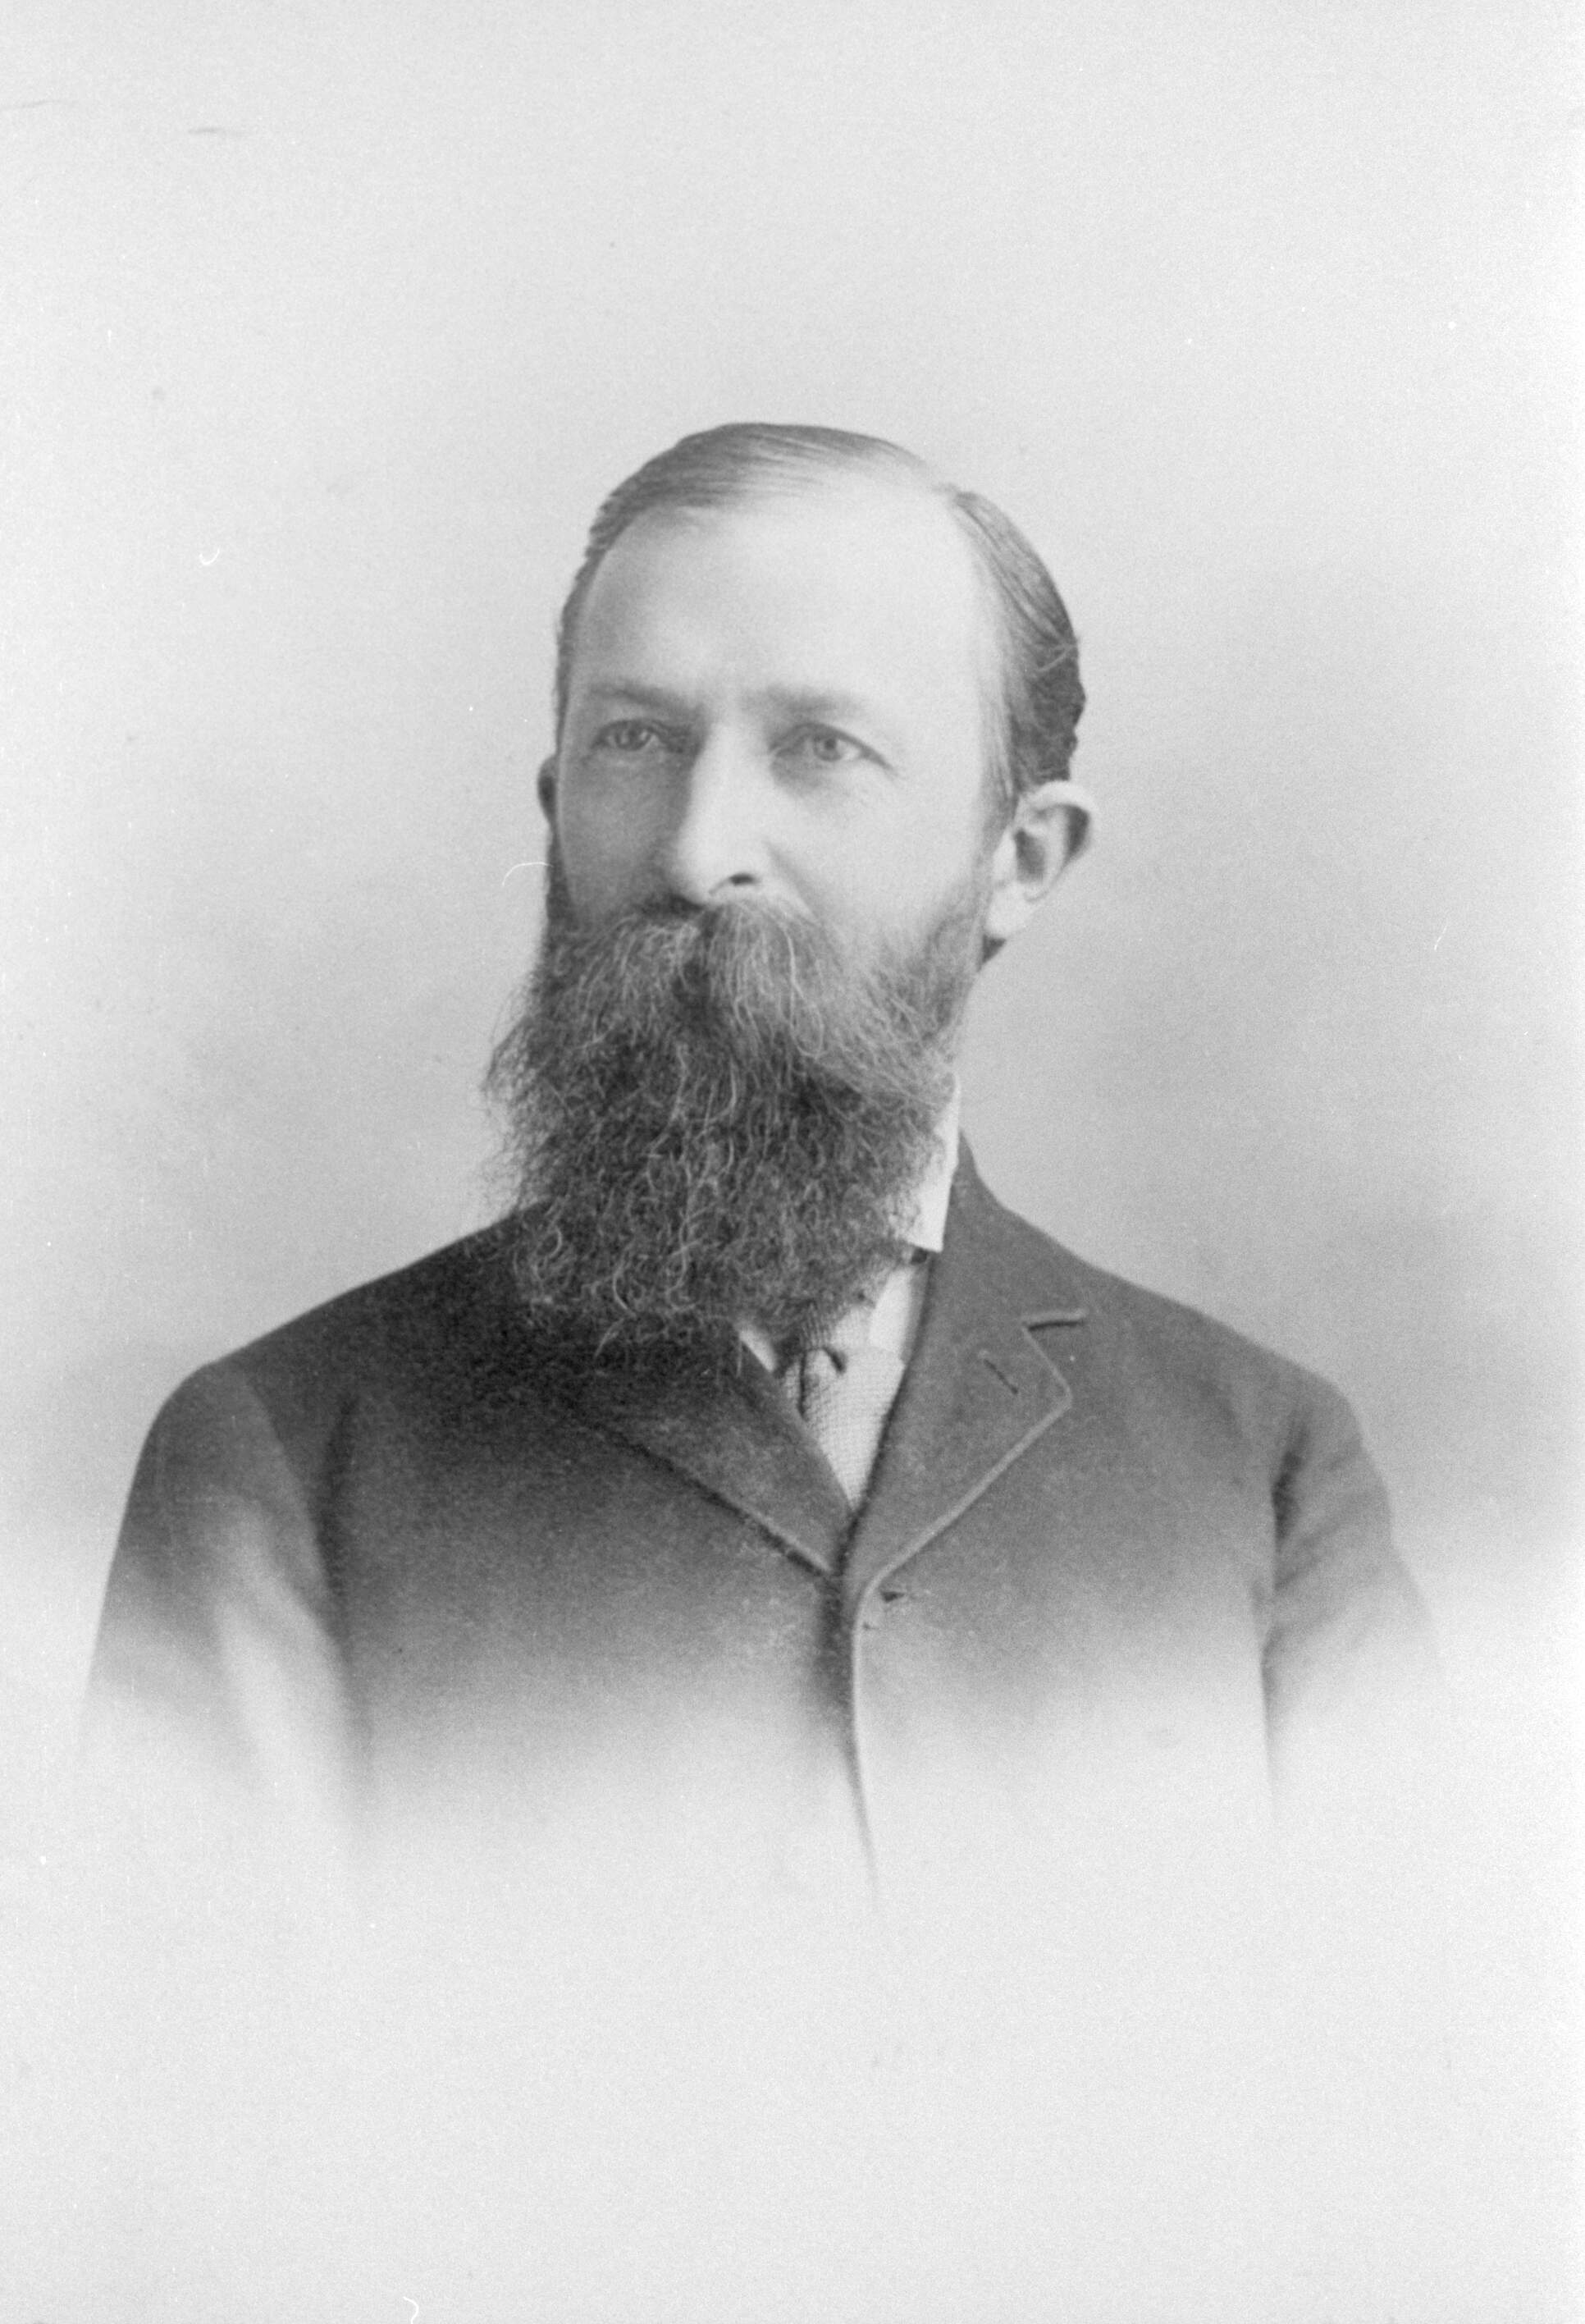
\includegraphics[width=1\linewidth]{images/john-h-kellogg.jpg}
    \caption*{John Harvey Kellogg (1852-1943)}
    \label{fig:john-h-kellogg}
\end{figure}

\egw{\textbf{Kitabu Hekalu Hai kina maoni ya uwongo, \underline{ya udanganyifu kuhusu ubinafsi wa Mungu na wa Kristo}}. Bwana alifungua mbele yangu maana halisi ya hisia hizi, akinionyesha kwamba ikiwa mafundisho haya hayatakataliwa kwa uthabiti, yanaweza kuwapoteza, kama yamkini, hata walio wateule. \textbf{Ukweli wa thamani na hisia nzuri ziliunganishwa na uwongo, nadharia potofu. Hivyo ukweli ulitumiwa kuthibitisha \underline{makosa ya hatari zaidi}. Vielelezo vya thamani vya Mungu vimefafanuliwa vibaya sana hivi kwamba vinaonekana kuunga mkono udanganyifu \underline{ulioasisiwa na yule muasi mkuu}. Hisia ambazo ni za ufunuo ya Mungu zimechanganyika na nadharia zenye udanganyifu za mashirika ya kishetani}.}[Lt146-1905.2; 1905][https://egwwritings.org/read?panels=p9430.8]

\egwnogap{Katika mabishano ya nadharia hizi \textbf{imedaiwa kwamba niliamini na kufundisha mambo yale yale} ambayo nimeagizwa kukemea katika kitabu Hekalu Hai. \textbf{Hili ninakataa}. Kwa jina la Yesu Kristo wa Nazareti, \textbf{nasema sivyo hivyo}.}[Lt146-1905.3; 1905][https://egwwritings.org/read?panels=p9430.9]

Mchanganyiko huu wa ukweli na makosa hufanya jambo kuwa gumu. Katika macho ya wataalamu wanaounga mkono utatu, tatizo linahusishwa tu na pantheism, na ushahidi wa imani ya Kellogg katika fundisho la Utatu linafasiriwa kuwa imani katika Utatu wa uwongo\footnote{Whidden, Woodrow W, et al. \textit{The Trinity : Understanding God's Love, His Plan of Salvation, and Christian Relationships}. Hagerstown, Md, Review And Herald Pub. Association, 2002., p. 217}. Karipio la Dada White linahusishwa na utetezi wa Utatu “sahihi,” ambao inasemekana aliamini. Kwa bahati mbaya, tafsiri kama hiyo haihusishi utetezi wa Dada White wa \emcap{Kanuni za Msingi} kuhusu \emcap{ubinafsi wa Mungu} na wa Kristo, hivyo ni tafsiri mbaya ya kazi yake. Katika sehemu zifuatazo, tutaangalia data ya kihistoria kuhusu uhusiano wa Dk. Kellogg na fundisho la Utatu kutoka kwa mtazamo wa ukweli wa Waadventista juu ya \emcap{ubinafsi wa Mungu}, ambao ulikuwa msingi wa imani yetu. Tukiwa na mtazamo huu, tunaamini kwamba data ya kihistoria itaangaza katika mwanga mpya na kuibua mazungumzo ya uaminifu na yenye kujenga katika kanisa letu.

\section*{Mawasiliano ya Dk. Kellogg na Ndugu Butler}

Katika sehemu ifuatayo tunawasilisha kwa ufupi mawasiliano yanayojulikana kati ya Dk. Kellogg na G. I. Butler juu ya kitabu, the Living Temple. Hapa, tunaona pingamizi ya Dk. Kellogg kuhusu mzozo huo. Alimwandikia Ndugu Butler:

\others{Kadiri ninavyoweza kufahamu, \textbf{utata} unaopatikana \textbf{katika ‘The Living Temple’,} \textbf{kwa ujumla jambo linaweza kuchemshwa hadi kwenye swali}: \textbf{\underline{Je, Roho Mtakatifu ni nafsi}?} Unasema hapana. Nilidhani kwamba Biblia ilisema hivi kwa sababu kiwakilishi cha kibinafsi ‘yeye’ kinatumika akizungumza juu ya Roho Mtakatifu. \textbf{Dada White anatumia kiwakilishi ‘yeye’ na amesema katika maneno mengi sana kwamba Roho Mtakatifu ni \underline{nafsi ya tatu ya Uungu}}. \textbf{Jinsi Roho Mtakatifu anaweza kuwa nafsi ya tatu na asiwe nafsi hata kidogo ni vigumu kwangu kuona}.}[Letter: J. H. Kellogg to G. I. Butler. Oct 28. 1903][https://static1.squarespace.com/static/554c4998e4b04e89ea0c4073/t/5db9fbc96defed1e45b497a4/1572469707862/1903-10-28-Kellog-to-Butler.pdf]

\begin{figure}[hp]
    \centering
    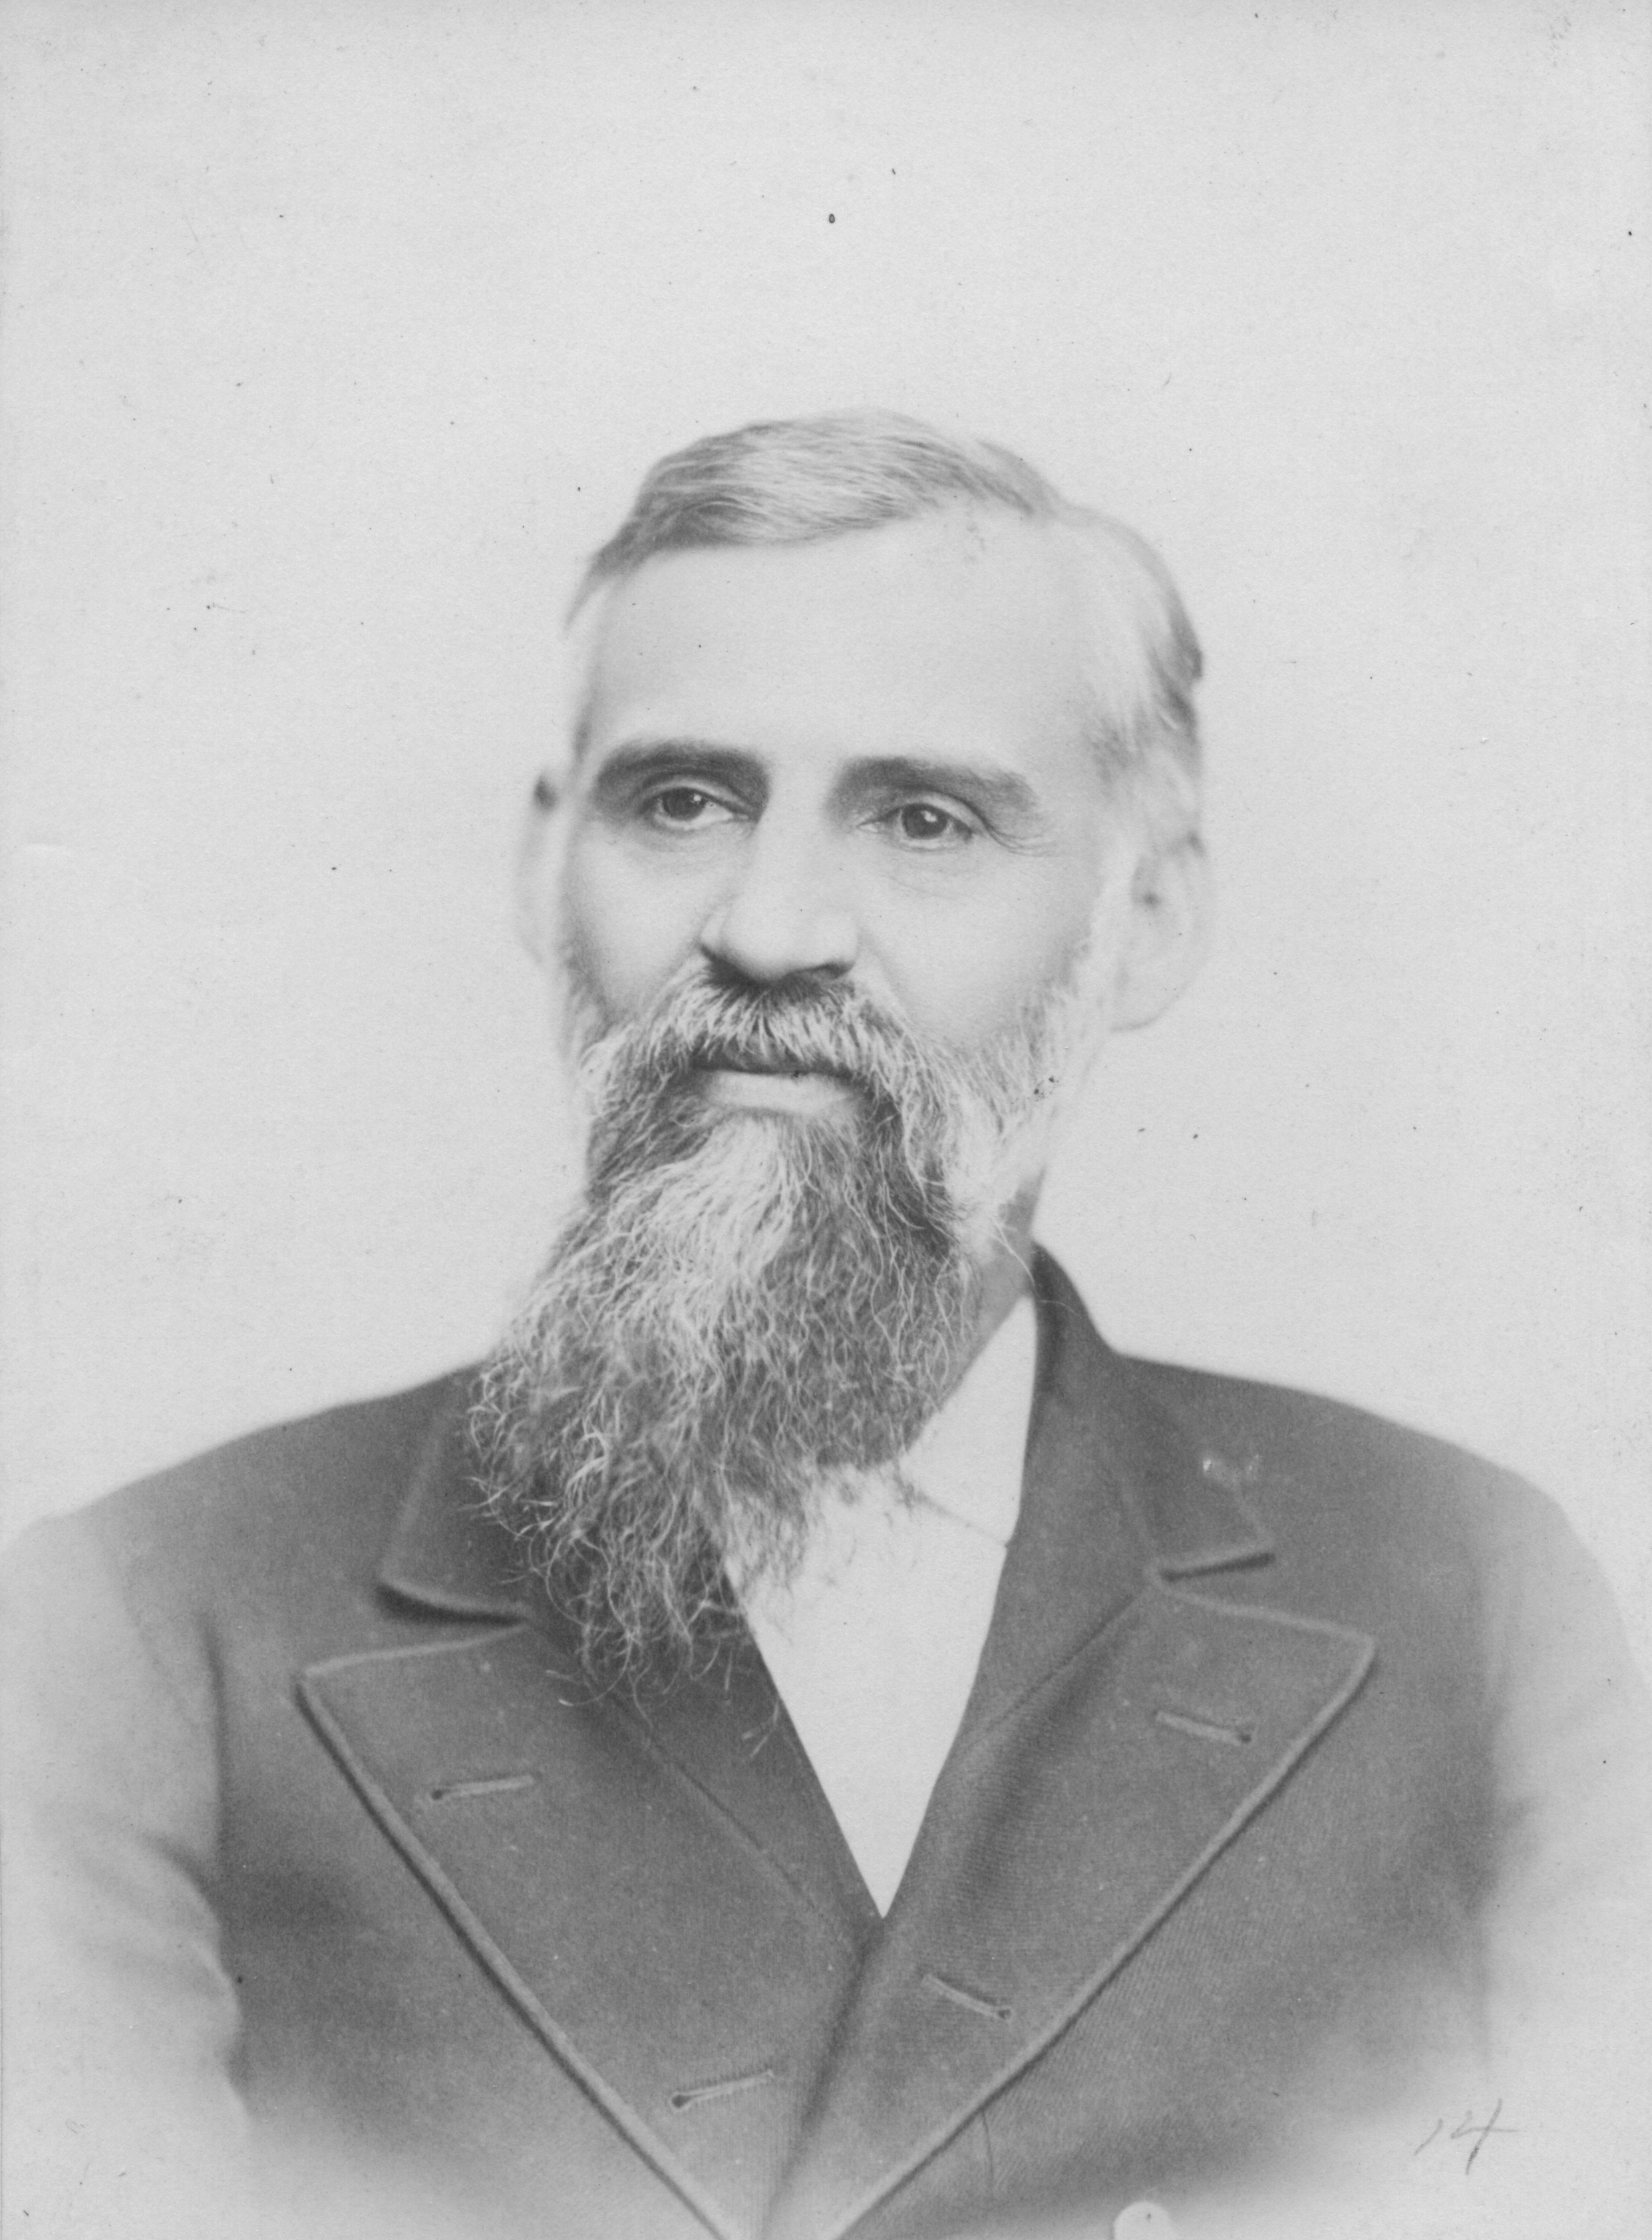
\includegraphics[width=1\linewidth]{images/george-ide-butler.jpg}
    \caption*{George Ide Butler (1834-1918)}
    \label{fig:g-i-butler}
\end{figure}

Kulingana na mtazamo wa Dk. Kellogg, tatizo zima la kitabu ‘The Living Temple’ inakuja kwa swali “\textit{Je! Roho Mtakatifu ni nafsi?}”. Ni wazi, yeye hatetei Mungu asiye na nafsi, kama anavyoshutumiwa mara nyingi\footnote{Whidden, Woodrow W, et al. \textit{The Trinity : Understanding God's Love, His Plan of Salvation, and Christian Relationships}. Hagerstown, Md, Review And Herald Pub. Association, 2002., p. 217}. Zaidi ya hayo, hata anaamini kwamba Roho Mtakatifu ni \textit{nafsi ya tatu ya Uungu}. Pia, anadai kwamba Ndugu Butler haamini kwamba Roho Mtakatifu ni nafsi. Tatizo ni wazi liko katika ufafanuzi wa neno \textit{‘nafsi’}. Katika hatua hii, Kellogg anaendelea:

\others{Ninaamini huyu Roho wa Mungu kuwa nafsi wewe huamini. Lakini hili ni swali tu la ufafanuzi. \textbf{Ninaamini Roho wa Mungu ni nafsi}; unasema, Hapana, sio nafsi. Sasa sababu pekee kwa nini tunatofautiana ni kwa sababu \textbf{tunatofautiana katika mawazo yetu kuhusu \underline{nini ni nafsi}}. \textbf{Wazo lako la nafsi labda ni la \underline{kufanana na mtu} au na binadamu}.}[Letter: J. H. Kellogg to G. I. Butler. Oct 28. 1903][https://static1.squarespace.com/static/554c4998e4b04e89ea0c4073/t/5db9fbc96defed1e45b497a4/1572469707862/1903-10-28-Kellog-to-Butler.pdf]

Ndugu Butler alijibu:

\others{\textbf{Ikiwa Dada White na wewe mko katika makubaliano kamili, itabidi niachane na hilo swala kabisa liwe kati yako na Dada White. \underline{Dada White anasema hakuna makubaliano kamilifu; unadai ipo}. \underline{Najua baadhi ya maandishi yake yanaonekana kukupa nguvu katika kudai kuwa anafanya hivyo}. Niko wazi vya kutosha kusema hivyo, lakini lazima nimpe nafasi yake mpaka akanushe kwa kusema kuna tofauti pia, na siamini unaweza kusema kikamilifu kile anachomaanisha. \underline{Mungu anakaa ndani yetu kwa Roho wake Mtakatifu}, kama Mfariji, kama Mkemeaji, hasa yule wa kwanza. Tunapokuja Kwake tunamshiriki yeye kwa sababu Roho hutoka Kwake; \underline{inatoka kwa Baba na Mwana}. Si nafsi anayetembea kwa miguu, au kuruka \underline{kama huluki halisi}, \underline{kwa maana yoyote kama Kristo na Baba walivyo} - angalau, ikiwa ni hivyo, ni zaidi ya ufahamu wangu wa maana ya lugha au maneno}.}[Letter: G. I. Butler to J. H. Kellogg. April 5. 1904]

Mawasiliano yaliyotolewa ni muhimu kwa kuelewa mgogoro wa Kellogg. Kellogg mwenyewe alisema, \others{jambo zima linaweza kuchambuliwa hadi kukifikia kiini chake kwa swali: \textbf{Je, Roho Mtakatifu ni nafsi?}} Vivyo hivyo Dk. Kellogg alimwandikia William White: \others{Nimekuwa nikisoma kwa makini sana kuona \textbf{ni nini kiini cha tatizo la Hekalu Hai}, na kadiri ninavyoweza kuona \textbf{\underline{swali zima} linajikita katika hili: \underline{Je, Roho Mtakatifu ni nafsi}?}}[Letter J. H. Kellogg to William White, October 28, 1903][https://drive.google.com/file/d/1\_S4S-Hc0K7Ka8gda9oRhPuAb9XzBTwmb/view] Je! hitimisho la Kellogg linaendeleaje kulinganishwa na mapitio na maelekezo ya asili ya mbinguni, ambayo yalituambia wazi kwamba mantiki katika Hekalu Hai ni \egwinline{si chochote ila ni dhana tu kuhusiana na \textbf{Umbile la Mungu na mahali uwepo wake ulipo}}[SpTB02 51.3; 1904][https://egwwritings.org/read?panels=p417.262]? Katika maandiko ya Ellen White na waanzilishi, neno ‘\textit{Umbile la Mungu}’ linahusu hasa Umbile la Baba. Kwa hiyo, kwa nini Kellogg anadai kwamba suala halisi ni Umbile la Roho Mtakatifu, wakati Mungu alionyesha kwamba suala linahusu Umbile la Baba?

Wengi wanadhani kwamba Dk. Kellogg anajaribu kudanganya, akikwepa suala la msingi. Hata hivyo, chini ya dhana fulani, hoja zake kuhusu Umbile la Roho Mtakatifu kimatiki zinaunga mkono maoni yake ya utata kuhusu \emcap{Umbile la Mungu}. Dhana hii inakuwa dhahiri ndani ya data yenyewe tunapofuata kwa makini mantiki yake.

Kama tulivyoona hapo awali, fundisho juu ya \emcap{Umbile la Mungu} linafundisha kwamba Mungu, Baba, ana umbo—mwili unaoonekana, wa dutu. Dk. Kellogg alikubali kwamba dai hili ni kweli ndani ya mipaka ya uelewa wetu finyu wa Mungu\footnote{\href{https://archive.org/details/J.H.Kellogg.TheLivingTemple1903/page/n33/}{Dr. John H. Kellogg, The Living Temple, p.31.}}. Hata hivyo, alihoji kwamba, kwa kweli, Mungu anazidi dhana zetu kuhusu umbo lake, kwani yuko nje ya vikwazo vya nafasi\footnote{\href{https://archive.org/details/J.H.Kellogg.TheLivingTemple1903/page/n33/}{Dr. John H. Kellogg, The Living Temple, p.33.}}. Kwa maana hii, Kellogg kwa kweli anaondoa uhalisia wa mwili wa kimwili, wa dutu wa Mungu. Dhana ambayo ingethibitisha mtazamo wa Dk. Kellogg ni \textit{ulinganifu wa kipekee} katika kuelewa \emcap{Umbile la Mungu} na lile la Roho Mtakatifu. Je, Roho Mtakatifu anazuiliwa na nafasi? Hapana, hazuiliwi. Je, Roho Mtakatifu ana mwili wa kimwili? Hapana! Kulingana na Yesu, \bible{kwa maana roho haina mwili wala mifupa}[Luka 24:39]. Je, Roho Mtakatifu ni nafsi? Jibu linategemea tafsiri yetu ya maana ya kuwa nafsi. Ni nini ubora au hali ya Roho Mtakatifu kuwa nafsi?\footnote{Matumizi ya moja kwa moja ya ufafanuzi wa neno ‘\textit{Umbile}’ kutoka \href{https://www.merriam-webster.com/dictionary/personality}{Kamusi ya Merriam Webster}} Tunapolinganisha imani ya Dk. Kellogg katika Umbile la Roho Mtakatifu na maoni ya Ndugu Butler, inakuwa dhahiri kwamba ubora wa Roho Mtakatifu kuwa nafsi hauendani na \others{ule wa \textbf{kufanana na mtu} au binadamu}. Butler alieleza wazi vigezo vyake kwa uamuzi huu\footnote{Katika barua yake kwa Dk. Kellogg, Ndugu Butler pia alidai kwamba hakuna tofauti kati ya nafsi na uwepo wa kimwili. Tazama \href{https://c7da.us/egwdl/Butler\%20to\%20Kellogg\%20Aug121904.pdf}{Barua kutoka Butler kwa Kellogg, Agosti 12, 1904, uk.6}}: \others{\textbf{Si nafsi anayetembea kwa miguu, au kuruka \underline{kama huluki halisi}, \underline{kwa maana yoyote kama Kristo na Baba walivyo} - angalau, ikiwa ni hivyo, ni zaidi ya ufahamu wangu wa maana ya lugha au maneno}}.

Je, umeona kwamba Ndugu Butler alishughulikia dhana ya Kellogg ambayo hakusema? Butler aliweka tofauti kati ya Baba na Kristo, kuhusiana na Roho Mtakatifu. Ndugu Butler yuko sahihi. Kuna tofauti kati ya Umbile la Roho Mtakatifu na lile la Mungu na Kristo. Kristo na Baba wana umbo la kimwili la mtu, wakati Roho Mtakatifu hana. Kuondoa umbo la kimwili la nafsi ya Baba ni \textit{kulinganisha kwa kipekee} uelewa wa Umbile la Baba na lile la Roho Mtakatifu. Mtazamo wa Kellogg ni wa kushawishi, kwa sababu uliungwa mkono na hoja halali kuhusu Umbile la Roho Mtakatifu.

Hebu tuchunguze kwa ufupi Umbile la Roho Mtakatifu. Ni nini ubora au hali ya Roho Mtakatifu kuwa nafsi?

\egw{\textbf{Roho Mtakatifu ana Umbile}, \textbf{\underline{vinginevyo} }Asingeweza \textbf{kushuhudia} kwa roho zetu na pamoja na roho zetu kwamba sisi ni watoto wa Mungu. \textbf{Lazima pia awe \underline{Nafsi ya kimungu}}, \textbf{\underline{vinginevyo}} Asingeweza \textbf{kuchunguza siri} zilizofichika \textbf{katika akili ya Mungu}.}[21LtMs, Ms 20, 1906, par. 32; 1906][https://egwwritings.org/read?panels=p14071.10296041&index=0]

\egw{\textbf{Roho Mtakatifu ni nafsi}; \textbf{\underline{kwa}} Yeye \textbf{hushuhudia} pamoja na roho zetu kwamba sisi ni watoto wa Mungu.}[21LtMs, Ms 20, 1906, par. 31; 1906][https://egwwritings.org/read?panels=p14071.10296040&index=0]

Sifa au hali zinazomfafanua Roho Mtakatifu kama nafsi zimetajwa wazi katika nukuu zilizotolewa. Hizi ni pamoja na uwezo wa kushuhudia na kuchunguza akili. Ushahidi zaidi unaweza kupatikana katika Maandiko, ambayo yanampa Roho Mtakatifu matendo kama vile kuzungumza (\textit{Matendo 13:2}), kufundisha (\textit{Yohana 14:26; 1 Wakorintho 2:13}), kufanya maamuzi (\textit{Matendo 15:28}), na kuwa na hisia (\textit{Waefeso 4:30}), miongoni mwa nyingine. Hizi \textit{sifa} kwa pamoja zinathibitisha Umbile la Roho Mtakatifu. Je, sifa hizi zinaweza kutumika pia kwa Baba na Mwana? Bila shaka. Hata hivyo, tofauti na Baba na Mwana, Roho Mtakatifu anatofautishwa kwa kukosa umbo la kimwili, linaloonekana. Wakati Ellen White alipomwuliza Kristo kuhusu \emcap{Umbile la Mungu}, swali lake hasa lililenga umbo la kibinafsi kama sifa inayofafanua Umbile la Baba.

\egw{Mara nyingi \textbf{nimemwona} Yesu mzuri, kwamba \textbf{Yeye ni nafsi}. \textbf{Nilimwuliza kama Baba Yake \underline{alikuwa nafsi} na \underline{alikuwa na umbo} kama Yeye}. Yesu alisema, ‘\textbf{Mimi ni chapa kamili ya Umbile la Baba yangu}.’}[EW 77.1; 1882][https://egwwritings.org/read?panels=p28.490&index=0]

Hii inatuleta kwenye tofauti kubwa katika jinsi Umbile la Roho Mtakatifu linavyoeleweka, tofauti na lile la Baba na Mwana. Ellen White anaelezea Roho Mtakatifu kama dhihirisho la kiroho la Kristo, akiweka mstari wazi kati ya dhihirisho la nje, linaloonekana la Kristo na dhihirisho lake la kiroho. Tofauti hii inasisitiza asili ya kipekee ya uwepo na utendaji wa Roho Mtakatifu duniani, tofauti na uwepo wa kimwili wa Kristo na Baba. Zingatia tofauti kati ya dhihirisho la nje, linaloonekana la Kristo, na dhihirisho lake la kiroho:

\egw{Kwamba \textbf{Kristo} angeweza \textbf{kujidhihirisha} kwao, na bado \textbf{asiwe anaonekana kwa ulimwengu}, ilikuwa siri kwa wanafunzi. Hawakuweza kuelewa \textbf{maneno ya Kristo katika \underline{maana yake ya kiroho}}. \textbf{Walikuwa wanafikiria \underline{dhihirisho la nje, linaloonekana}}. Hawakuweza kuelewa ukweli kwamba wangeweza kuwa na \textbf{uwepo wa Kristo pamoja nao}, na \textbf{bado Yeye asionekane na ulimwengu}. \textbf{Hawakuelewa maana ya \underline{dhihirisho la kiroho}}.}[ST November 18, 1897, par. 6; 1897][https://egwwritings.org/read?panels=p820.14727&index=0]

Roho Mtakatifu si nafsi kwa maana ya kimwili bali anadhihirishwa kwa maana ya kiroho. Ikiwa uelewa wa kipekee wa Umbile la Roho Mtakatifu utatumika kwa Baba, basi kwa matokeo yake umbo lake la kimwili la nafsi linaondolewa. Umbile lake linafanywa kuwa la kiroho. Hii ndiyo sababu Ellen White alitaja mtazamo wa Kellogg kama umizimu. Je, unajua fundisho gani, hasa, lina kanuni kuu, kwamba Baba na Roho Mtakatifu ni sawa katika Umbile lao? Ni \textit{fundisho la utatu}. Je, inawezekana kwamba Dk. Kellogg alikuwa kwa kweli anainua upande wa kitheolojia wa maswali ya utatu?

\section*{Ungamo la Kellogg kuhusu Hekalu Hai}

Katika mahojiano yake na G. W. Amadon na A. C. Bourdeau, mwezi mmoja baada ya kutengwa na ushirika, alikiri kwamba bila kukusudia alileta upande wa kitheolojia wa swali la Utatu katika kitabu chake “The Living Temple”.

\others{\textbf{Sasa, nilifikiri nilikuwa nimeondoa kabisa upande wa kitheolojia wa maswali ya \underline{utatu na aina hiyo ya mambo}}. \textbf{Sikukusudia \underline{kuiweka ndani} hata kidogo}, na nilichukua tahadhari kueleza katika dibaji kwamba sikufanya hivyo. Sikuwahi kufikiri chochote kuhusu \textbf{swali lolote la kitheolojia} \textbf{\underline{kuletwa ndani yake}}. Nilitaka tu kuonyesha kwamba \textbf{moyo haupigi kwa mwendo wake bali kwamba ni uweza wa Mungu unaoufanya uendelee}.}[Kellogg vs. The Brethren: His Last Interview as an Adventist, p. 58.][https://forgotten-pillar.s3.us-east-2.amazonaws.com/1990\_kellogg\_vs\_brethren\_lastInterview\_oct7\_1907\_spectrum\_v20\_n3-4.pdf]

Kama tungetafuta katika kitabu chake maneno ya utatu, hatungepata yoyote. Je! hilo lingekuwa ushahidi kwamba Kellogg hana ufahamu katika kukiri kwake? Kitu pekee tunachopata ni mafundisho ambayo yanaondoka kutoka kwenye msingi wa imani yetu—\emcap{kanuni za kimsingi}—kuhusu \emcap{ubinafsi wa Mungu} na mahali uwepo wake ulipo. Semi za utatu hazipo hapo bali hisia zake kuhusu \emcap{ubinafsi wa Mungu} zinapatana na hisia za utatu kuhusu ubinafsi wa Mungu. Hisia hizi ni za udanganyifu na Kellogg alikemewa kwayo. Alipotaka kueleza kwa uwazi imani katika fundisho la Utatu, kwa matumaini ya kurekebisha kitabu, alikemewa tena kwa maneno, \egwinline{\textbf{Nadharia za kiraka} haziwezi kukubaliwa na wale walio waaminifu kwa imani} na kwa \emcap{Kanuni za Msingi}\footnote{\href{https://egwwritings.org/?ref=en_Lt253-1903.28&para=9980.36}{EGW, Lt253-1903.28; 1903}}. Tatizo la muhimu la fundisho la Utatu, kuhusiana na \emcap{ubinafsi wa Mungu}, ndilo dhana ya msingi ambayo wote Tatu, Baba, Mwana, na Roho Mtakatifu, wana aina moja ya ubinafsi hivi kwamba Hao hujumuisha Mungu mmoja. Katika mwanga huu, tunaweza kuelewa madai ya Kellogg juu ya ubinafsi wa Roho Mtakatifu, kwamba Roho Mtakatifu ni nafsi ya tatu ya Uungu. Dk. Kellogg alimnukuu Ellen White wakati akisisitiza madai yake; ingawa alitumia maneno sawa, alikuwa na hisia mbaya. Kwa kuzingatia kukiri kwa Dk. Kellogg, kwa kujumuisha \others{\textbf{upande wa kitheolojia wa maswali ya \underline{utatu}}}, na madai yake kwamba \others{\textbf{jambo zima inaweza kuchambuliwa hadi swali}: \textbf{\underline{Je, Roho Mtakatifu ni nafsi}}?}, tunaweza kuona dhana fiche kwamba Baba na Mwana ni Nafsi kwa njia sawa na Roho Mtakatifu. Hii ndiyo sababu Ndugu Butler alimwandikia kuhusu ubinafsi wa Roho Mtakatifu: \others{\textbf{Siyo Nafsi anayetembea kwa miguu, au kuruka \underline{kama huluki halisi}, \underline{sawia na jinsi Kristo na Baba walivyo} – angalau, ikiwa ni, ni zaidi ya ufahamu wangu ya maana ya lugha au maneno.}}[Letter from G. I. Butler to J. H. Kellogg, April 5 1904.]

\section*{Uwepo wa Mungu unadhihirika katika asili}

Kutoka kwa kazi za waanzilishi wetu, tumeona kwamba ubinafsi wa Roho Mtakatifu zaidi imeonyeshwa wazi katika suala la uwepo wa Mungu. Dada White alituambia kwamba Hekalu Hai \egwinline{hutanguliza yale ambayo si chochote ila ni dhana tu kuhusiana na \textbf{ubinafsi wa Mungu na mahali ambapo uwepo wake upo}.}[SpTB02 51.3; 1904][https://egwwritings.org/read?panels=p417.262] \emcap{Ubinafsi wa Mungu} na mahali palipo na uwepo wake ni mafundisho mawili yanayojumuisha pande zote; mmoja inathibitisha nyingine. Kataa moja, unakana lingine. Dhana hii inaonekana wazi katika kitabu, Hekalu Hai. Katika sehemu zilizopita, tunasoma hoja za Kellogg za \emcap{ubinafsi wa Mungu} zilizochukuliwa kutoka katika kitabu chake. Alipinga kuwa haina maana kuzungumza kuhusu umbo la Mungu au namna yoyote inayoonekana. Alikana ukweli wa Mungu kama nyenzo iliyo dhahiri na huluki anayeonekana. Ikiwa Mungu ni roho, hana umbo wala mwili, basi hasitiriwi katika uwepo wake kwa eneo moja; Haya ndiyo maoni ambayo Kellogg aliyatetea katika Hekalu Hai.

\others{Mmoja husema, ‘\textbf{Mungu anaweza kuwapo kwa Roho wake, au kwa nguvu zake, lakini \underline{hakika Mungu mwenyewe} hawezi kuwapo kila mahali mara moja kwa wakati mmoja}.’ Tunajibu: Nguvu inaweza kuwaje kutengwa na chanzo cha nguvu? \textbf{Ambapo Roho wa Mungu anafanya kazi}, ambapo kuna nguvu za Mungu iliyodhihirika, \textbf{Mwenyezi Mungu \underline{yumo} na hakika yuko}…}[John H. Kellogg, The Living Temple, p.28.][https://archive.org/details/J.H.Kellogg.TheLivingTemple1903/page/n29/]

Wakati Dk. Kellogg aliandika \others{Anasema mmoja, ‘Mungu anaweza kuwa kwa Roho Wake…‘}, alirejelea hisia za mapainia wetu ambao walikuwa waaminifu kwa \emcap{Kanuni za Msingi}. Hapa ndipo mahali dhahiri ambapo Dk. Kellogg aliondoka kutoka kwenye \emcap{Kanuni za Msingi}. Je, hatua hii inapatana na fundisho la Utatu? Tukichunguza msimamo wetu wa sasa katika Mafundisho za Kimsingi \#2, tunaona kwamba Mungu mmoja, kama umoja wa nafsi tatu, hayupo kila mahali kupitia wakala wa Roho Mtakatifu, bali yupo kila mahali kwa Nafsi yake.

\others{Kuna \textbf{Mungu mmoja}: Baba, Mwana, na Roho Mtakatifu, \textbf{umoja wa} \textbf{Nafsi} tatu zenye umilele sawa. Mungu ni asiyekufa, mwenye nguvu zote… na \textbf{yupo kila mahali}.}[Fundamental Beliefs of Seventh-day Adventist, \#2 Trinity; 2020 Edition][https://www.adventist.org/wp-content/uploads/2020/06/ADV-28Beliefs2020.pdf]

\section*{Mtazamo wa Dk. Kellogg kuhusu Mungu}

Katika kuchunguza mzozo uliozunguka Hekalu Hai, tunaona kweli kwamba Dk. Kellogg aliibua \others{upande wa kitheolojia wa maswali ya utatu.}[Kellogg vs. The Brethren: His Last Interview as an Adventist, p. 58.][https://forgotten-pillar.s3.us-east-2.amazonaws.com/1990\_kellogg\_vs\_brethren\_lastInterview\_oct7\_1907\_spectrum\_v20\_n3-4.pdf] Swali lingine tunaloibua katika kuchunguza hisia za Kellogg na \emcap{Kanuni za Msingi} ni nani anayerejelea kwa maneno “\textit{Mungu mmoja}”? Hakuna data ya kujibu swali hilo moja kwa moja, lakini kuna data nyingi zinazoonyesha kwamba uelewa wa Dk. Kellogg wa “\textit{Mungu mmoja}” ulikuwa uelewa wa Utatu. Barua yake kwa W. W. Prescott ni ushahidi mmoja unaoonyesha dhana hiyo:

\others{Tofauti ni hii: \textbf{Tunaposema Mungu} yumo kwenye mti, neno ‘\textbf{Mungu}’ \textbf{linafahamika katika maana yake pana zaidi}, na watu wanaelewa maana kuwa \textbf{Uungu} umo kwenye mti, \textbf{Mungu Baba, Mungu Mwana, na Mungu Roho Mtakatifu}, ambapo uelewa sahihi ili \textbf{dhana nzuri} zihifadhiwe katika akili zetu, ni kwamba Mungu Baba anaketi kwenye kiti chake cha enzi mbinguni ambapo Mungu Mwana pia yupo; \textbf{wakati uhai wa Mungu, au roho au uwepo ni nguvu inayoenea kila mahali ambayo inatekeleza mapenzi ya Mungu katika ulimwengu wote}.}[Letter: Dr. Kellogg to Prof. W. W. Prescott, Oct. 25, 1903][https://forgotten-pillar.s3.us-east-2.amazonaws.com/1903-10-25-JHKellogg-to-W.W.Prescott.pdf]

Katika sura inayofuata, tutawasilisha hoja yetu: ikiwa \others{dhana nzuri} ya Mungu iliyotetewa na Dk. Kellogg ilikuwa kweli, basi ufafanuzi wake wa Roho Mtakatifu kuwa \others{uhai wa Mungu, au roho au uwepo ni nguvu inayoenea kila mahali ambayo inatekeleza mapenzi ya Mungu katika ulimwengu wote} ungetatua kweli ugumu wote wa Hekalu Hai. Lakini haikuwa hivyo. Tatizo la kweli la Dk. Kellogg lilikuwa mtazamo wake wa Mungu, na msimamo wake wa utatu haukutatua tatizo halisi—\emcap{ubinafsi wa Mungu}.

Kuna barua nyingine inayofichua ikituonyesha matokeo ya kuinua \others{upande wa kitheolojia wa maswali ya utatu.} Akiandika kwa rafiki yake Dk. Hayward, Dk. Kellogg alitafakari:

\others{\textbf{Wanatheolojia hawa} wametafuta kufifisha akili za watu na kufanya \textbf{ukweli huu mtamu na mzuri \underline{uonekane wa kuchukiza} kwao, kwa kuingiza ndani yake \underline{mgogoro wa zamani kuhusu Utatu}}.}

\othersnogap{Sijawahi kuuliza swali kuhusu \textbf{sehemu gani ya Mungu ipo ndani ya mwanadamu}, kama ni \textbf{Mungu, Baba}; \textbf{Mungu, Mwana}; au \textbf{Mungu, Roho Mtakatifu}. Jambo pekee lilikuwa kwamba ni Mungu na sio mwanadamu.}[Letter: Dr. J. H. Kellogg to Dr. Hayward, Aug., 15. 1905][https://forgotten-pillar.s3.us-east-2.amazonaws.com/1903-08-15-kellogg-to-hayward.pdf]

Hapa tunaona mvutano kati ya Dk. Kellogg na baadhi ya wanatheolojia wa Waadventista Wasabato wa wakati huo, ambapo \others{ukweli mtamu na mzuri} wa Dk. Kellogg kuhusu uwepo wa kimungu wa Mungu ulisukwa na \others{mgogoro wa zamani kuhusu Utatu}. Hii inatuambia kwamba katika siku za Dk. Kellogg, fundisho la Utatu lilikuwa la utata, na kwa hakika halikuchukuliwa kama kitu chema, bali kama kitu ambacho kilifanya mafundisho ya Kellogg \others{ya kuchukiza}. Lakini ni akina nani hawa wanatheolojia ambao Dk. Kellogg aliwataja? Hakutaja mtu yeyote katika barua yake kwa Dk. Hayward, lakini tunaweza kupata wazo la \others{wanatheolojia hawa} kulingana na barua yake iliyotumwa siku 10 kabla kwa I. G. Butler\footnote{\href{https://forgotten-pillar.s3.us-east-2.amazonaws.com/1905-08-05-kellogg-butler.pdf}{Letter: J. H. Kellogg to I. G. Butler, Aug., 5. 1905}}, akitoa masikitiko yake kuhusu ushindani wa Kongamano Kuu naye. Hawa walikuwa A. G. Daniells, W. C. White, na W. W. Prescott. Tunaweza pia kumjumuisha G. I. Butler mwenyewe katika kundi hilo, kwani yeye pia alikuwa mwanatheolojia aliyeshiriki katika \others{mgogoro wa zamani kuhusu Utatu}. Wote hawa walikuwa na nafasi za uongozi ndani ya kanisa la Waadventista Wasabato, na wote walikuwa wasio-Watatu. Hoja inatolewa kwamba tatizo la mafundisho ya Dk. Kellogg liko mahali pengine kuliko maoni yake ya utatu, kwa sababu inasemekana kanisa lilikuwa la utatu wakati huo, na inasemekana Ellen White alikuwa mwamini utatu mwenyewe. \footnote{Hii kwa sasa ni hadithi maarufu inayoendelezwa na walei.} Kama hii ilikuwa hivyo, na katika mchanganyiko huu wa ukweli na makosa, je, hatupaswi kuwa na angalau utetezi wa fundisho la utatu, kulichambua kutoka kwenye makosa? Hatujapata data yoyote kama hiyo. Badala yake, data zote tulizonazo ni katika utetezi wa \emcap{Kanuni za Msingi}, na fundisho juu ya uwepo na \emcap{Umbile la Mungu}, ambayo yote yanapinga fundisho la Utatu. Ellen White alisema kuhusu ukweli: fundisho la Utatu \egwinline{haliwezi kukubaliwa na wale ambao ni \textbf{waaminifu kwa imani na kwa kanuni} ambazo zimestahimili upinzani wote wa nguvu za kishetani.}[Lt253-1903.28; 1903][https://egwwritings.org/read?panels=p14068.9980036]

Katika tafakari hii fupi juu ya tofauti kati ya maoni ya Dk. Kellogg na \emcap{Kanuni za Msingi} ambayo aliondoka kwayo, tunaweza kutambua sifa zifuatazo ambazo zinafanana na fundisho la Utatu:

\begin{itemize}
    \item Neno ‘Mungu’ linawakilisha dhana kamili ya Mungu kama Mungu Baba, Mungu Mwana, na Mungu Roho Mtakatifu.
    \item Mungu yupo kila mahali kwa Nafsi yake.
    \item Ubora au hali ya Baba kuwa nafsi inasawazishwa na ile ya Roho Mtakatifu.\footnote{\href{https://www.adventist.org/wp-content/uploads/2020/06/ADV-28Beliefs2020.pdf}{Mafundisho za Kimsingi \#5}: \others{Yeye \normaltext{[Roho Mtakatifu]} \textbf{ni nafsi} \underline{kama} walivyo \textbf{Baba} na Mwana}; \href{https://www.adventist.org/wp-content/uploads/2020/06/ADV-28Beliefs2020.pdf}{Mafundisho za Kimsingi \#3}: \others{\textbf{Sifa} na nguvu \textbf{zinazoonyeshwa katika} Mwana na \textbf{Roho Mtakatifu ni \underline{pia} zile za Baba}}}
\end{itemize}

Sifa hizi tatu za maoni ya Dk. Kellogg zinaondoka kutoka kwenye msingi wa imani yetu—\emcap{Kanuni za Msingi}—lakini zinapatana na mafundisho ya Utatu. Kwa kusema hivi, hatudai kwamba Dk. Kellogg anawajibika kwa kukubaliwa kwa fundisho la Utatu katika safu zetu, bali kwamba fundisho la Utatu lilikuwa haki ya Kellogg ya kuondoka kutoka kwenye msingi wa imani yetu, ulioanzishwa mwanzoni mwa kazi yetu. Tatizo la kweli lilikuwa \textit{kuondoka} kutoka kwenye \emcap{kanuni za msingi}, na Dk. Kellogg pamoja na sisi kama kanisa tumefanya hatua hizo. Tofauti ni kwamba Dk. Kellogg aliishia kwenye pantheism, wakati sisi tuliishia kwenye nukta \#2 ya Mafundisho za Kimsingi.

Katika sura ifuatayo, tutachunguza mafundisho ya Dk. Kellogg kwamba Mungu hutegemeza uhai wote, na jinsi ukweli huu, ukichanganywa na mtazamo wa uwongo wa Mungu na Umbile lake, ulimfanya awe mpantheisti.

% Dr. Kellogg and the Trinity doctrine

\begin{titledpoem}
    
    \stanza{
        In Kellogg's quest, a question posed, \\
        "Is the Holy Ghost, indeed, a person enclosed?" \\
        A controversy stirred, the essence debated, \\
        The Trinity's mystery, intricately related.
    }

    \stanza{
        Kellogg questioned beyond the tangible, the seen, \\
        Where the Holy Spirit's form has never been. \\
        A spiritual essence, not bound by space, \\
        Challenging the Father's physical embrace.
    }

    \stanza{
        The Holy Ghost, a person, yet not in form, \\
        In actions, emotions, a divine norm. \\
        Witnessing, teaching, decisions so clear, \\
        A presence felt, though not seen near.
    }

    \stanza{
        Butler contrasted, in physical sense, \\
        The Father and Christ, their presence immense. \\
        Yet, the Spirit's persona, distinct in its role, \\
        A spiritual manifestation, completing the whole.
    }

    \stanza{
        Ellen asked of Jesus, if His Father's form was like His own, \\
        "In my Father's image," He replied, in a tone so gently sown. \\
        Yet, the Spirit, in essence, a guiding light, \\
        Not seen, but felt, in the believers' sight.
    }

    \stanza{
        A doctrine emerges, the Trinity's core, \\
        Equal in personalities, yet so much more. \\
        Kellogg's perspective, once seen as stray, \\
        Raises the question, in a theological way.
    }

    \stanza{
        Yet, Scripture guides, through mystery's veil, \\
        Revealing God's form, where human views fail. \\
        The Father, embodied, a truth we embrace, \\
        While the Spirit's presence, a formless grace.
    }

    \stanza{
        In divine revelation, the answers found, \\
        God's personality, in Scripture, profound. \\
        The Father, in form; the Spirit, without, \\
        In this, the Bible resolves all doubt.
    }
\end{titledpoem}

